\documentclass[crop=false,class=book]{standalone}
\RequirePackage{etex}
\usepackage{geometry}
\geometry{a4paper, margin = 1.0in}
\usepackage[utf8]{inputenc}
\usepackage[english]{babel}
\usepackage[dvipsnames]{xcolor}
\usepackage{graphicx}
\usepackage{listings}
\usepackage{mathtools}
\usepackage{amsfonts,amsthm,esint,mathrsfs}
\usepackage{paracol}
\usepackage{wrapfig}
\usepackage[nottoc]{tocbibind}
\usepackage{natbib}
\usepackage[font={scriptsize,it}]{caption}
\usepackage{float}
\usepackage{multicol}
\setlength{\multicolsep}{6.0pt plus 2.0pt minus 1.5pt}
\usepackage[font={scriptsize}]{subcaption}
\usepackage{pgfplots,tikz,tkz-euclide}
\usetikzlibrary{calc,patterns,angles,quotes,arrows,arrows.meta,shapes,shapes.geometric,cd,hobby,positioning,decorations.markings}
\usetkzobj{all}
\pgfplotsset{compat=1.9}
\usepackage{hyperref}
\usepackage[toc,acronym,nogroupskip]{glossaries}
\hypersetup{colorlinks=true,linkcolor=blue,filecolor=magenta,urlcolor=Cerulean,citecolor=SkyBlue}
\usepackage{enumitem}
\usepackage{upgreek}
\graphicspath{{../images/}}
%-------------Tikz Presets----------%
\pgfdeclareradialshading{myring}{\pgfpointorigin}{color(0cm)=(transparent!0);color(5mm)=(pgftransparent!50);color(1cm)=(pgftransparent!100)}
\pgfdeclarefading{ringo}{\pgfuseshading{myring}}
%------------Theorem Styles---------%
\newtheoremstyle{mystyle}{0.1em}{0pt}{}{}{\bfseries}{}{.5em}{}
\theoremstyle{mystyle}
\newtheorem{theorem}{Theorem}[section]
\newtheorem{definition}{Definition}[section]
\newtheorem{lemma}{Lemma}[section]
\newtheorem{corollary}{Corollary}[section]
\newtheorem{proposition}{Proposition}[section]
\newtheorem{example}{Example}[section]
\newtheorem{problem}{Problem}[section]
\newtheorem{question}{Question}[section]
\newtheorem{remark}{Remark}[section]
\newtheorem{properties}{Properties}[section]
\newtheorem{notation}{Notation}[section]
\newtheorem{axiom}{Axiom}[section]
\newtheorem*{theorem*}{Theorem}
\newtheorem*{definition*}{Definition}
\newtheorem*{properties*}{Properties}
\newtheorem*{remark*}{Remark}
%--------Declared Math Operators----%
\DeclareMathOperator{\Refl}{Refl}
\DeclareMathOperator{\Span}{Span}
\DeclareMathOperator{\sgn}{sgn}
\DeclareMathOperator{\multideg}{mutlideg}
\DeclareMathOperator{\GCD}{GCD}
\DeclareMathOperator{\LC}{LC}
\DeclareMathOperator{\LT}{LT}
\DeclareMathOperator{\Tr}{Tr}
\DeclareMathOperator{\LM}{LM}
\DeclareMathOperator{\rk}{rk}
\DeclareMathOperator{\nul}{nul}
\DeclareMathOperator{\LCM}{LCM}
\DeclareMathOperator{\Mon}{Mon}
\DeclareMathOperator{\Spec}{Spec}
\DeclareMathOperator{\proj}{proj}
\DeclareMathOperator{\comp}{comp}
\DeclareMathOperator{\sinc}{sinc}
%-------------New Commands----------%
\DeclarePairedDelimiter\norm{\lVert}{\rVert}
\DeclarePairedDelimiter\ceil{\lceil}{\rceil}
\DeclarePairedDelimiter\floor{\lfloor}{\rfloor}
\renewcommand*{\glstextformat}[1]{\textcolor{RoyalBlue}{#1}}
\renewcommand{\glsnamefont}[1]{\textbf{#1}}
\renewcommand\labelitemii{$\circ$}
\renewcommand\thesubfigure{\arabic{chapter}.\arabic{figure}.\arabic{subfigure}}
%---------------GLOSSARY------------%
\makeglossaries
\loadglsentries{../glossary}
\loadglsentries{../acronym}
%--------------Title Page-----------%
\setlength{\parindent}{0em}
\setlength{\parskip}{0em}
\setenumerate{itemsep=0pt,topsep=2pt}
\pagenumbering{arabic}
\begin{document}
\chapter{Master's Work}
\section{Preliminaries}
\subsection{Set Theory}
\begin{definition}
A set is a collection of distinct objects, none of which are the set itself.
\end{definition}
\begin{remark}
As neither "Collection," nor "Objects," have been define, the above definition is logically meaningless.
\end{remark}
\begin{definition}
The objects in a set are called the elements of the set. If $x$ is an element of $A$, we write $x\in A$.
\end{definition}
\begin{definition}
The empty set $\emptyset$ is the set containing no elements. It is unique.
\end{definition}
\begin{definition}
A set $A$ is said to be a subset of a $B$ if and only if $x\in A\Rightarrow x\in B$. This is denoted $A\subset B$.
\end{definition}
\begin{corollary}
For any set $A$, $\emptyset \subset A$ and $A\subset A$.
\end{corollary}
\begin{proof}
Suppose not. Then $\exists x\in \emptyset: x\notin A$. A contradiction. Suppose $A\not\subset A$. Then $\exists x\in A:x\notin A$, a contradiction.
\end{proof}
\begin{definition}
$A\subset B$ is said to be a proper subset of $B$ if and only if there is an $x\in B$ such that $x\notin A$.
\end{definition}
\begin{definition}
Two sets $A$ and $B$ are said to be equal if and only if $x\in A \Leftrightarrow x\in B$.
\end{definition}
\begin{theorem}
Two sets $A$ and $B$ are equal if and only if $A\subset B$ and $B\subset A$.
\end{theorem}
\begin{proof}
$[A=B]\Leftrightarrow\big[[x\in A \Rightarrow x\in B]\big]\land \big[[y\in B \Rightarrow y\in A]\big]\Leftrightarrow [A\subset B\land B\subset A]$. 
\end{proof}
\begin{definition}
If $A$ and $B$ are sets, then $B\setminus A = \{x\in B:x\notin A\}$. This is called the set difference.
\end{definition}
\begin{theorem}
If $A$ and $B$ are sets and $A\subset B$, then $B\setminus(B\setminus A)=A$.
\end{theorem}
\begin{proof}
$[x\in B\setminus(B\setminus A)]\Rightarrow [x\in B \land x\notin \{x\in B:x\notin A\}]\Rightarrow [x\in A\subset B]$. $[x\in A]\Rightarrow [x\notin B\setminus A]\Rightarrow [x\in B\setminus(B\setminus A)]$.
\end{proof}
\begin{definition}
The universe set is the set under consideration from which all subsets are drawn.
\end{definition}
\begin{definition}
If $\mathcal{U}$ is a universe set, $A\subset \mathcal{U}$, then the complement of $A$ is $\mathcal{U}\setminus A$ and is denoted $A^c$.
\end{definition}
\begin{remark}
The previous theorem shows that $(A^c)^c = A$.
\end{remark}
\begin{definition}
If $A$ and $B$ are sets, then $A\cup B = \{x: x\in A \lor x\in B\}$ is called their union.
\end{definition}
\begin{corollary}
If $A$ and $B$ are sets, then $A\subset A\cup B$.
\end{corollary}
\begin{proof}
$[x\in A]\Rightarrow [x\in A\lor x\in B]\Rightarrow [x\in A\cup B]$.
\end{proof}
\begin{theorem}
If $A$ and $B$ are sets, $A=A\cup B$ if and only if $B\subset A$.
\end{theorem}
\begin{proof}
$[B\subset A]\Rightarrow \big[[x\in A\cup B] \Rightarrow [x\in A]\big]\Rightarrow[A\cup B \subset A], [A\subset A\cup B]\Rightarrow[A=A\cup B]$. $[x\in B] \Rightarrow [x\in A\cup B]\Rightarrow [x\in A]$
\end{proof}
\begin{definition}
If $A$ and $B$ are sets, then $A\cap B = \{x:x\in A \land x\in B\}$ is called their intersection.
\end{definition}
\begin{corollary}
If $A$ and $B$ are sets, $A\cap B \subset A$ and $A\cap B \subset B$.
\end{corollary}
\begin{proof}
$[x\in A\cap B]\Rightarrow [x\in A\land x\in B]\Rightarrow \big[[A\cap B \subset A]\land [A\cap B \subset B]\big]$.
\end{proof}
\begin{theorem}
If $A$ and $B$ are sets, then $A=A\cap B$ if and only if $A\subset B$.
\end{theorem}
\begin{proof}
$[A=A\cap B]\Rightarrow [x\in A\Rightarrow x\in A \cap B]\Rightarrow [x\in B]$. $[A\subset B]\Rightarrow [x\in A\Rightarrow x\in B]\Rightarrow [x\in A\cap B]\Rightarrow [A=A\cap B]$.
\end{proof}
\begin{theorem}
If $A,B$, and $C$ are sets, then the following are true:
\begin{enumerate}
\item $A\cap (B\cup C) = (A\cap B)\cup (A\cap C)$
\item $A\cup (B\cup C) = (A\cup B)\cap (A\cup C)$
\end{enumerate}
\end{theorem}
\begin{proof}
In order,
\begin{enumerate}
\item $[x\in A\cap (B\cup C)]\Rightarrow \big[[x\in A] \land [x\in B\cup C]\big]\Rightarrow \big[[x\in A\land x\in B]\lor [x\in A\land x\in C]\big]\Rightarrow [x\in (A\cap B)\cup (A\cap C)]$. $[x\in (A\cap B)\cup(A\cap C)]\Rightarrow \big[[x\in A\land x\in C]\lor [x\in A \land x\in C]\big]\Rightarrow \big[[x\in A]\land [x\in B\lor x\in C]\big]\Rightarrow [x\in A\cap(B\cup C)]$.
\item $[x\in A\cup (B\cap C)]\Rightarrow \big[[x\in A]\lor [x\in B\cap C]\big] \Rightarrow \big[[x\in A \lor x\in B]\land [x\in A$ or $x\in C]\big]\Rightarrow [x\in (A\cap B)\cup (A\cap C)]$. $[x\in (A\cup B)\cap (A\cup C)]\Rightarrow \big[[x\in A\lor B]\land [x\in A\lor B]\big]\Rightarrow \big[[x\in A]\lor[x\in B\land C]\big]\Rightarrow [x\in A\cap(B\cup C)]$.
\end{enumerate}
\end{proof}
\begin{theorem}[DeMorgan's Laws]
If $A$ and $B$ are subsets of some universe $\mathcal{U}$, then the following are true:
\begin{enumerate}
\item $(A\cup B)^c = A^c \cap B^c$
\item $(A\cap B)^c = A^c \cup B^c$
\end{enumerate}
\end{theorem}
\begin{proof}
In order,
\begin{enumerate}
\item $[x\in (A\cup B)^c]\Rightarrow [x\in A^c\land x\in B^c]\Rightarrow [x\in A^c\cap B^c]$. $[x\in A^c \cap B^c]\Rightarrow [x\in A^c\land x\in B^c]\Rightarrow [x\notin A\cup B]\Rightarrow [x\in (A\cup B)^c]$.
\item $[x\in (A\cap B)^c]\Rightarrow [x\in A^c\lor x\in B^c]\Rightarrow [x\in A^c \cup B^c]$. $[x\in A^c \cup B^c]\Rightarrow [x\notin A\lor x\notin B]\Rightarrow [x\notin A\cap B]\Rightarrow [x\in (A\cap B)^c]$.
\end{enumerate}
\end{proof}
\begin{definition}
If $A$ is a set and $a,b\in A$, then the ordered pair $(a,b)$ is the set $\{\{a\},\{a,b\}\}$.
\end{definition}
\begin{remark}
This definition is due to Kuratowski. Note that $(a,b)$ and $(b,a)$ are not necessarily equal.
\end{remark}
\begin{definition}
The Cartesian Product of $A$ and $B$ is defined as $A\times B = \{(a,b):a\in A, b\in B\}$.
\end{definition}
\begin{definition}
The power set of a set $A$ is the set $\mathcal{P}(A) = \{\mathcal{U}:\mathcal{U}\subset A\}$. That is, it is the set of all subsets of $A$.
\end{definition}
\subsection{Algebra}
\begin{definition}
If $A$ is a set, a relation $R$ on $A$ is a subset of $A\times A$. If $a,b\in A$ and $(a,b)\in R$, we write $aR b$.
\end{definition}
\begin{remark}
For a relation $R$ it is not necessary true that $aRb$ implies $bRa$, nor is it necessarily true that $aRa$.
\end{remark}
\begin{definition}
A relation $R$ on a set $A$ is said to be reflexive if and only if $\forall a\in A$, $aRa$.
\end{definition}
\begin{definition}
A relation $R$ on a set $A$ is said to be symmetric if and only if $\forall a,b\in A$, $aRb\Leftrightarrow bRa$.
\end{definition}
\begin{definition}
A relation $R$ on a set $A$ is said to be transitive if and only if $\forall a,b,c\in A$, $aRb \land bRc \Rightarrow aRc$.
\end{definition}
\begin{definition}
A relation $R$ on a set $A$ is said to be asymmetric if and only if $\forall a,b\in A$, $(a,b)\in R\Rightarrow (b,a) \notin R$.
\end{definition}
\begin{definition}
A relation on $R$ is said to be total if and only if $\forall a,b \in A$, either $aRb$, $bRa$, or both.
\end{definition}
\begin{definition}[Relation of Equality]
Equality is a relation with the following properties:
\begin{enumerate}
\item Equality is Reflexive: $a=a$ for all $a\in A$.
\item Equality is Symmetric: $a=b$ if and only if $b=a$.
\item Equality is Transitive: If $a=b$ and $b=c$, then $a=c$.
\item The relation is uniquely defined by the set $\{(a,a)\in A\times A:a\in A\}$.
\end{enumerate}
\end{definition}
\begin{definition}
A relation $R$ on a set $A$ is said to be antisymmetric if and only if $\forall a,b \in A$, $aRb\land bRa\Rightarrow a=b$.
\end{definition}
\begin{definition}
A function $f:A\rightarrow B$ is a subset of $A\times B: \forall a\in A$, $\exists b\in B: (a,b)\in f$ and $[(a,b)\in f\land (a,c)\in f]\Leftrightarrow [b=c]$. The image of $a\in A$ is the unique $b\in B:(a,b)\in f$, denoted $a\mapsto b$ or $f(a)=b$. Functions are also called maps/mappings.
\end{definition}
\begin{definition}
An indexing set is a set whose elements label some other set.
\end{definition}
\begin{example}
If $A$ is an indexing set, then $\{\mathcal{U}_{\alpha}:\alpha \in A\}$ is a set of elements $\mathcal{U}_{\alpha}$, and there is one for each $\alpha \in A$.
\end{example}
\begin{axiom}
If $X$ is a set of nonempty sets $\mathcal{U}_{\alpha}$, indexed over $A$, then $\exists f:X\rightarrow \underset{\alpha \in A}\cup \mathcal{U}_{\alpha}$ such that $f(\mathcal{U}_{\alpha}) \in \mathcal{U}_{\alpha}$, $\forall \alpha\in A$.
\end{axiom}
\begin{remark}
This is called the axiom of choice. It is a blatantly obvious statement, however many of the results it gives are far from intuitive. For those interested, the axiom of choice is consistent with modern set theory (Called Zermelo-Fraenkel set theory, or ZF). It may thus be rejected or accepted without logical contradiction. We shall accept it.
\end{remark}
\begin{definition}
If $f:A\rightarrow B$ and if $\mathcal{O}\subset A$, then the image of $\mathcal{O}$ under $f$ is the set $f(\mathcal{O}) = \{f(a)\in B:a\in \mathcal{O}\}$.
\end{definition}
\begin{definition}
If $f:A\rightarrow B$ and $\mathscr{O}\subset B$, the preimage is the set $f^{-1}(\mathscr{O}) = \{x\in A:f(x)\in \mathscr{O}\}$.
\end{definition}
\begin{corollary}
If $f:A\rightarrow B$, $f(\emptyset) = f^{-1}(\emptyset) = \emptyset$.
\end{corollary}
\begin{proof}
$[y\in f(\emptyset)]\Rightarrow [\exists x\in \emptyset:f(x)=y]$. A contradiction. Therefore, etc.
\end{proof}
\begin{theorem}
If $f:A\rightarrow B$, $B_1\subset B$, then $f(f^{-1}(B_1))\subset B_1$.
\end{theorem}
\begin{proof}
$[f(x)\in f(f^{-1}(B_1))]\Rightarrow [x\in f^{-1}(B_1)]\Rightarrow [f(x)\in B_1]$.
\end{proof}
\begin{theorem}
If $f:A\rightarrow B$, $A_1\subset A$, then $A_1\subset f^{-1}(f(A_1))$.
\end{theorem}
\begin{proof}
$[x\in A_1]\Rightarrow [f(x) \in f(A_1)]\Rightarrow x\in f^{-1}(f(A_1))$.
\end{proof}
\begin{theorem}
If $f:A\rightarrow B$, $A_1\subset A$, then $f(A_1) = \emptyset \Leftrightarrow A_1 = \emptyset$.
\end{theorem}
\begin{proof}
If $A_1 = \emptyset$, we are done. If not, let $x\in A_1$. Then $f(x)\in f(A_1)$, and thus $f(A_1)\ne \emptyset$. Therefore, etc.
\end{proof}
\begin{corollary}
If $f:A\rightarrow B$, $A_1\subset A_2\subset A$, then $f(A_1)\subset f(A_2)$.
\end{corollary}
\begin{proof}
$[y\in f(A_1)]\Rightarrow[\exists x\in A_1:f(x)=y]\Rightarrow [x\in A_2] \Rightarrow [f(x)\in f(A_2)]$
\end{proof}
\begin{corollary}
If $f:A\rightarrow B$, $B_1\subset B_2\subset B$, then $f^{-1}(B_1)\subset f^{-1}(B_2)$.
\end{corollary}
\begin{proof}
$[x\in f^{-1}(B_1)] \Rightarrow [f(x) \in B_1] \Rightarrow [f(x) \in B_2]\Rightarrow [x\in f^{-1}(B_2)]$.
\end{proof}
\begin{theorem}
If $f:A\rightarrow B$, $A_1,A_2\subset A$, then $f(A_1 \cup A_2) = f(A_1)\cup f(A_2)$.
\end{theorem}
\begin{proof}
$[y\in f(A_1\cup A_2)]\Rightarrow [\exists x\in A_1 \cup A_2:y=f(x)]\Rightarrow [y \in f(A_1)\cup f(A_2)]$. $[y\in f(A_1)\cup f(A_2)]\Rightarrow \big[[\exists x\in A_1] \lor [\exists x\in A_2]: y=f(x)\big]\Rightarrow [x\in A_1\cup A_2]\Rightarrow [f(x)\in f(A_1\cup A_2)]$
\end{proof}
\begin{theorem}
If $f:A\rightarrow B$, $A_1,A_2\subset A$, then $f(A_1\cap A_2)\subset f(A_1)\cap f(A_2)$.
\end{theorem}
\begin{proof}
$[y\in f(A_1 \cap A_2)]\Rightarrow [\exists x\in A_1 \cap A_2:y=f(x)]\Rightarrow [x\in A_1 \land x \in A_2] \Rightarrow[y \in f(A_1)\cap f(A_2)]$.
\end{proof}
\begin{theorem}
If $f:A\rightarrow B$, $B_1,B_2\subset B$, then $f^{-1}(B_1\cup B_2) = f^{-1}(B_1)\cup f^{-1}(B_2)$.
\end{theorem}
\begin{proof}
$[x\in B_1\cup B_2]\Rightarrow [f(x)\in B_1\cup B_2]\Rightarrow [f(x)\in B_1\lor f(x)\in B_2]\Rightarrow [x\in f^{-1}(B_1)\cup f^{-1}(B_2)]$. $[x \in f^{-1}(B_1)\cup f^{-1}(B_2)]\Rightarrow [f(x)\in B_1\lor f(x) \in B_2]\Rightarrow [f(x) \in B_1\cup B_2]\Rightarrow [x\in f^{-1}(B_1\cup B_2)]$.
\end{proof}
\begin{theorem}
If $f:A\rightarrow B$, $B_1,B_2\subset B$, then $f^{-1}(B_1\cap B_2) = f^{-1}(B_1)\cap f^{-1}(B_2)$.
\end{theorem}
\begin{proof}
$[x\in f^{-1}(B_1\cap B_2)]\Rightarrow [f(x) \in B_1 \cap B_2]\Rightarrow [f(x)\in B_1\land f(x) \in B_2 ]\Rightarrow [x\in f^{-1}(B_1)\cap f^{-1}(B_2)]$. $[x\in f^{-1}(B_1)\cap f^{-1}(B_2)]\Rightarrow [x\in f^{-1}(B_1)\land x\in f^{-1}(B_2)]\Rightarrow [f(x) \in B_1\land f(x) \in B_2]\Rightarrow [f(x)\in B_1\cap B_2]\Rightarrow [x\in f^{-1}(B_1\cap B_2)]$.
\end{proof}
\begin{theorem}
If $f:A\rightarrow B$, $B_1 \subset B$, then $f^{-1}(B\setminus B_1) = f^{-1}(B)\setminus f^{-1}(B_1)$.
\end{theorem}
\begin{proof}
$[x\in f^{-1}(B\setminus B_1)]\Leftrightarrow [f(x)\notin B_1]\Leftrightarrow [x\in f^{-1}(B)\setminus f^{-1}(B_1)]$
\end{proof}
\begin{remark}
If $f:A\rightarrow B$, the image of $A$ under $f$ is often called the range (A is often called the domain).
\end{remark}
\begin{definition}
A function $f:A\rightarrow B$ is said to be injective if and only if $\big[[(a,b)\in f]\land[(a',b)\in f]\big]\Leftrightarrow [a=a']$.
\end{definition}
\begin{definition}
If $f:A\rightarrow B$ is injective, then the inverse $f^{-1}:f(A)\rightarrow A$ is defined by $f^{-1}(y)=x:y=f(x)$.
\end{definition}
\begin{definition}
A function $f:A\rightarrow B$ is said to be surjective if and only if $f(A) = B$.
\end{definition}
\begin{definition}
A function is said to be bijective if and only if it is injective and surjective.
\end{definition}
\begin{theorem}
If $f:A\rightarrow B$ is bijective, then $f^{-1}$ is bijective.
\end{theorem}
\begin{proof}
$[f^{-1}(y_1) = f^{-1}(y_2)]\Rightarrow [\exists x\in A:[f(x) = y_1]\land [f(x)=y_2]]\Rightarrow [y_1=y_2]$. By definition, $f^{-1}$ is surjective.
\end{proof}
\begin{definition}
If $f:A\rightarrow B$ and $g:B\rightarrow C$, then $g\circ f:A\rightarrow C$ is defined by the image $g(f(x)), x\in A$. 
\end{definition}
\begin{theorem}
If $f:A\rightarrow B$, $g:B\rightarrow C$, and $\mathcal{V}\subset C$, then $(g\circ g)^{-1}(\mathcal{V}) = f^{-1}(g^{-1}(\mathcal{V}))$.
\end{theorem}
\begin{proof}
$[x\in (g\circ f)^{-1}(\mathcal{V})]\Leftrightarrow [g(f(x))\in \mathcal{V}] \Leftrightarrow [f(x)\in g^{-1}(\mathcal{V})]\Leftrightarrow [x\in f^{-1}(g^{-1}(\mathcal{V}))]$.
\end{proof}
\begin{theorem}
If $f:A\rightarrow B$ is bijective, $g:B\rightarrow C$ is bijective, then $g\circ f$ is bijective.
\end{theorem}
\begin{proof}
$\big[[f(A) = B]\land [g(B) = C]\big]\Rightarrow [g(f(A)) = g(B) = C]$. $[g(f(x_1))=g(f(x_2))]\Leftrightarrow [f(x_1)=f(x_2)]\Leftrightarrow [x_1=x_2]$.
\end{proof}
\begin{theorem}
If $f:A\rightarrow B$ is bijective, $A_1\subset A$, and $f(A_1) = B$, then $A_1=A$.
\end{theorem}
\begin{proof}
$\Big[\big[[A_1^c \ne \emptyset]\Rightarrow [f(A_1^c) \ne \emptyset]\big]\land[f(A_1)\cap f(A_1^c) = \emptyset]\Big]\Rightarrow [\exists y\in B:y\notin f(A_1)]$, a contradiction.
\end{proof}
\begin{definition}
If $A$ is a set, then a binary operation $*$ on the set $A$ is a function from $A\times A$ to $A$.
\end{definition}
\begin{definition}
A binary operation $*$ is said to be associative if and only if $a*(b*c) = (a*b)*c$.
\end{definition}
\begin{definition}
An element $e\in A$ is said to be an identity element if and only if for all $a\in A$, $e*a = a*e = a$.
\end{definition}
\begin{definition}
An element $b\in A$ is said to be an inverse of $a$ if and only if $a*b=b*a = e$. We write $b=a^{-1}$
\end{definition}
\begin{definition}[Group]
A group is a set $G$ with a binary operation $*$, denoted $\langle G,* \rangle$, with the following properties: 
\begin{enumerate}
\item There exists an identity element $e$.
\item For every element $a\in A$, there is an inverse element.
\item The binary operation $*$ is associative.
\end{enumerate}
\end{definition}
\begin{remark}
Note that it is not necessarily true that $a*b = b*a$. These are special groups (Abelian Groups).
\end{remark}
\begin{theorem}
If $\langle G, * \rangle$ is a group and $e$ is the identity, then it is unique.
\end{theorem}
\begin{proof}
For suppose $e'$ is an identity element not equal to $e$. But $e' = e'*e  = e$. A contradiction. Thus, $e$ is unique.
\end{proof}
\begin{theorem}
If $\langle G, * \rangle$ is a group and $a\in G$, then $a^{-1}\in G$ is unique.
\end{theorem}
\begin{proof}
$a'^{-1} = a'^{-1}*e = a'^{-1}(a*a^{-1}) = (a'^{-1}*a)*a^{-1} = e*a^{-1} = a^{-1}$. Thus, $a^{-1}$ is unique.
\end{proof}
\begin{corollary}
The identity element of a group is its own inverse.
\end{corollary}
\begin{proof}
For $e=e*e = e$. As inverses are unique, $e=e^{-1}$.
\end{proof}
\begin{theorem}
If $\langle G,*\rangle$ is a group and $a,b\in G$, then $(a*b)^{-1} = b^{-1}*a^{-1}$.
\end{theorem}
\begin{proof}
$(a*b)*(b^{-1}*a^{-1}) = a*(b*b^{-1})*a^{-1} = a*a^{-1} = e=b^{-1}*b=b^{-1}*(a^{-1}*a)*b=(b^{-1}*a^{-1})*(a*b)  $.
\end{proof}
\begin{theorem}
If $\langle G,* \rangle$ is a group and $a\in G$, then $(a^{-1})^{-1} = a$.
\end{theorem}
\begin{proof}
For $a^{-1}*(a^{-1})^{-1} = (a^{-1}* a)^{-1} = e$, and $(a^{-1})^{-1}*a^{-1} = (a*a^{-1})^{-1} = e$. From uniqueness, $(a^{-1})^{-1} = a$.
\end{proof}
\begin{definition}
If $\langle G, * \rangle$ and $\langle G',\circ \rangle$ are groups and $f:G\rightarrow G'$ is a bijective function, then $f$ is said to be an isomorphism between $\langle G, * \rangle$ and $\langle G',\circ \rangle$ if and only if for all $a,b\in G$, $f(a*b) =f(a)\circ f(b)$.
\end{definition}
\begin{definition}
$\langle G, *\rangle$ and $\langle G', \circ \rangle$ are said to be isomorphic if and only if there is an isomorphism between them.
\end{definition}
\begin{theorem}
If $\langle G, * \rangle$ and $\langle G', \circ \rangle$ are isomorphic with identities $e_*$ and $e_{\circ}$ are the identities, then $f(e_*) = e_{\circ}$.
\end{theorem}
\begin{proof}
$\forall a\in G,\ f(a)=f(a* e_*) = f(a)\circ f(e_*)$ as $f$ is an isomorphism. As identities are unique, $f(e_*) = e_{\circ}$.
\end{proof}
\begin{theorem}
If $\langle G, * \rangle$ and $\langle G', \circ \rangle$ are isomorphic, with isomorphism $f$, and if $a\in G$, then $f(a^{-1}) = f(a)^{-1}$.
\end{theorem}
\begin{proof}
For $e_{\circ}=f(e_*) = f(a*a^{-1}) = f(a^{-1}*a) = f(a)\circ f(a^{-1})=f(a^{-1})\circ f(a)$. As inverses are unique, $f(a^{-1})=f(a)^{-1}$.
\end{proof}
\begin{definition}
A binary operation $*$ on a set $A$ is said to be commutative if and only for all $a,b\in A$, $a*b = b*a$.
\end{definition}
\begin{definition}
A field is a set $F$ with two operations $+$ and $\cdot$, denoted $\langle F, +,\cdot \rangle$, with the following properties:
\begin{enumerate}
\item $a+b=b+a$ \hfill [Addition is Commutative]
\item $a+(b+c)=(a+b)+c$ \hfill [Addition is Associative]
\item $a\cdot b = b\cdot a$ \hfill [Multiplication is Commutative]
\item $a\cdot (b\cdot c) = (a\cdot b)\cdot c$ \hfill [Multiplication is Associative]
\item There is a $0\in F$ such that $0+a=a$ for all $a\in F$ \hfill [Existence of Additive Identity]
\item There is a $1\in F$ such that $1\cdot a = a$ for all $a\in F$ \hfill [Existence of Multiplicative Identity]
\item For each $a\in F$ there is a $b\in F$ such that $a+b = 0$. $b$ is denoted $-a$ \hfill [Existence of Additive Inverses]
\item For each $a\in F$, $a\ne 0$ there is a $b\in F$ such that $a\cdot b = 1$. $b$ is denoted $a^{-1}$. \hfill [Existence of Multiplicative Inverses]
\item $a\cdot(b+c) = a\cdot b + a\cdot c$ \hfill [Distributive Property]
\end{enumerate}
\end{definition}
\begin{definition}
A subfield of a field $\langle F,+,\cdot \rangle$ is a set $K\subset F$, such that $\langle K, +,\cdot \rangle$ is a field.
\end{definition}
\begin{theorem}
In a field, $0$ and $1$ are unique.
\end{theorem}
\begin{proof}
For suppose not, and let $0'$ and $1'$ be other identities. Then $1'=1'\cdot 1 = 1$ and $0'=0'+0=0$.
\end{proof}
\begin{theorem}
For any field $\langle F,+,\cdot \rangle$, for any $a\in F$, $a\cdot 0 = 0$.
\end{theorem}
\begin{proof}
For $0 = a\cdot 0 + (-a\cdot 0) = a\cdot(0+0) +(-a\cdot 0) = a\cdot 0 + a\cdot 0 + (-a\cdot 0) = a\cdot 0$. Thus, $a\cdot 0 = 0$.
\end{proof}
\begin{remark}
If $1=0$, then $a=a\cdot 1 = a\cdot 0 = 0$, and thus every element is zero. A very boring field.
\end{remark}
\begin{corollary}
In a field $\langle F, +,\cdot \rangle$, if $0\ne 1$, then $0$ has no inverse.
\end{corollary}
\begin{proof}
For let $a$ be such an inverse. Then $a\cdot 0 = 1$. But for any element of $F$, $a \cdot 0 = 0$. But $0\ne 1$, a contradiction.
\end{proof}
\begin{theorem}
If $a+b = 0$, then $b= (-1)\cdot a$ where $(-1)$ is the solution to $1+(-1)=0$.
\end{theorem}
\begin{proof}
$a+(-1)a = a(1+(-1)) = a\cdot 0 = 0$. From uniqueness, $b=(-1)a$. We may thus write additive inverses as $-a$
\end{proof}
\begin{definition}
Given two fields $\langle F,+,\cdot \rangle$ and $\langle F', +',\times \rangle$, a bijection function $f:F\rightarrow F'$ is said to be a field isomorphism if and only if for all elements $a,b\in F$, $f(a+b)=f(a)+'f(b)$, and $f(a\cdot b) = f(a)\times f(b)$
\end{definition}
\begin{definition}
$\langle F,+,\cdot \rangle$ and $\langle F', +',\times \rangle$, are said to be isomorphic if and only if they have an isomorphism.
\end{definition}
\begin{theorem}
Given an ismorphism between two fields $\langle F,+,\cdot \rangle$ and $\langle F', +',\times \rangle$, $f(1) = 1'$ and $f(0) = 0'$.
\end{theorem}
\begin{proof}
For let $x\in F$. Then $f(x)=f(x\cdot 1) = f(x)\times f(1)$, and $f(x)=f(x+0) = f(x)+'f(0)$. Therefore, etc.
\end{proof}
\begin{theorem}
In a field $\langle F,+,\cdot \rangle$, $(a+ b)^2 = a^2 + 2ab + b^2$ ($2$ being the solution to $1+1$).
\end{theorem}
\begin{proof}
For $(a+b)^2 = (a+b)(a+b) = a(a+b)+b(a+b) = a^2 + ab + ba + b^2 = a^2 +ab(1+1)+b^2 = a^2 + 2ab + b^2$.
\end{proof}
\subsection{Relations of Order}
\begin{definition}
Given a set $A$, a total order on $A$ is a relation $\leq$ with the following properties: For all $a,b,c\in A$,
\begin{enumerate}
    \item $a\leq b$ and $b\leq a$ if and only if $a=b$.\hfill [Antisymmetry]
    \item If $a\leq b$ and $b\leq c$, then $a\leq c$. \hfill [Transitivity]
    \item Either $a\leq b$, or $b\leq a$, or both. \hfill [Totality]
\end{enumerate}
\end{definition}
\begin{remark}
If $a\leq b$, we may also write $b\geq a$.
\end{remark}
\begin{definition}
Given a set $A$, a strict relation of order is a relation $<$ with the following properties: For all $a,b,c\in A$,
\begin{enumerate}
    \item Precisely one of the following is true: $a<b$, $b<a$, $a=b$. \hfill [Trichotomy]
    \item If $a<b$ and $b<c$, then $a<c$. \hfill [Transitivity]
\end{enumerate}
\end{definition}
\begin{definition}
An ordered field is a field $\langle F,+,\cdot \rangle$ with a total order $\leq$ with the following properties: For all $a,b,c\in F$,
\begin{enumerate}
    \item If $a\leq b$, then $a+c\leq b+c$
    \item If $0 \leq a$ and $0\leq b$, then $0\leq a\cdot b$
    \item $0\leq 1$
\end{enumerate}
\end{definition}
\begin{remark}
If $a\leq b$ and $a\ne b$, we write $a<b$.
\end{remark}
\begin{theorem}
In a field, $(ab)^2 = a^2b^2$.
\end{theorem}
\begin{proof}
For $(ab)^2 = (ab)(ab)=(a)(b)(a)(b)= (a)(a)(b)(b)=a^2b^2$.
\end{proof}
\begin{theorem} In an ordered field, if $0\leq a$ and $0\leq b$, then $0\leq a+b$.
\end{theorem}
\begin{proof}
For as $0\leq a$, $0+b\leq a+b$. But $0+b = b$ and $0\leq b$. From transitivity, $0\leq a+b$.
\end{proof}
\begin{theorem}
In an ordered field, if $0\leq x$, then $-x\leq 0$.
\end{theorem}
\begin{proof}
For $0\leq x$, and thus $(-x)=0+(-x)\leq x+(-x) =0$. From transitivity, $(-x)\leq 0$.
\end{proof}
\begin{theorem}
In a field, $(-1)^2 = 1$.
\end{theorem}
\begin{proof}
For $(-1)^2 +(-1) = (-1)(-1+1) = (-1)\cdot 0 = 0$. As additive inverses are unique, $(-1)^2 = 1$.
\end{proof}
\begin{theorem}
In an ordered field, $0\leq x^2$.
\end{theorem}
\begin{proof}
If $0 \leq x$, we are done. Suppose $x\leq 0$. Then $0\leq (-x) = (-1)x$, and thus $0\leq (-1)^2 x^2=x^2$
\end{proof}
\begin{theorem}
In an ordered field, $a\leq b$ if and only if $0 \leq b-a$
\end{theorem}
\begin{proof}
For suppose $a\leq b$. Then $0=a+(-a)\leq b-a\Rightarrow 0 \leq b-a$. If $0\leq b-a$, then $a=0+a \leq (b-a)+a = b\Rightarrow a\leq b$.
\end{proof}
\begin{corollary}
If $a\leq b$, then $-b\leq -a$.
\end{corollary}
\begin{proof}
For then $0 \leq b-a$, and thus $-(b-a)=a-b\leq 0$, and therefore $-b \leq -a$.
\end{proof}
\begin{theorem}
In an ordered field, if $a\leq b$ and $c\leq d$, then $a+c \leq b+d$.
\end{theorem}
\begin{proof}
For $0\leq b-a$ and $0\leq d-c$. Thus, $0\leq (b-a)+(d-c)= (b+d)-(a+c)$, and therefore $a+c \leq b+d$.
\end{proof}
\begin{theorem}
In an ordered field, if $0\leq a$ and $b\leq 0$, then $ab\leq 0$.
\end{theorem}
\begin{proof}
For as $b\leq 0$, $0\leq -b$, and thus $0\leq -ba$, and therefore $-(-ba) = ba \leq 0$.
\end{proof}
\begin{theorem}
If $0< a$, then $0<\frac{1}{a}$.
\end{theorem}
\begin{proof}
For $\frac{1}{a}\ne 0$ as it is invertible, and $0$ is not. But $0\leq1=a\cdot \frac{1}{a}$ and $0<a$ and thus $\frac{1}{a} \not <0$. Therefore $0<\frac{1}{a}$.
\end{proof}
\begin{theorem}
In an ordered field, if $0<a\leq b$, then $0<\frac{1}{b}\leq\frac{1}{a}$.
\end{theorem}
\begin{proof}
As $a\leq b$, $\frac{1}{b}=a\cdot \frac{1}{ba} \leq b\cdot \frac{1}{ba}=\frac{1}{a}$. Thus, $0< \frac{1}{b}\leq \frac{1}{a}$.
\end{proof}
\begin{theorem}
In an ordered field, if $0 \leq a \leq b$, then $a^2 \leq b^2$.
\end{theorem}
\begin{proof}
For as $0\leq a \leq b$, $a\cdot a \leq b\cdot a$. Thus, $a^2 \leq b \cdot a$. But also $a\cdot b \leq b\cdot b$. Thus, $a\cdot b \leq b^2$. By transitivity, $a^2 \leq b^2$.
\end{proof}
\begin{corollary}
If $1\leq a$, then $a \leq a^2$. If $0\leq a \leq 1$, then $a^2 \leq a$.
\end{corollary}
\begin{proof}
For as $1\leq a$, $a=1\cdot a \leq a^2$. If $0\leq a \leq 1$, then $a^2 \leq 1\cdot a = a$.
\end{proof}
\subsection{The Real Numbers}
We construct the "God-Given" positive integers $\mathbb{N}$, then the whole numbers $\mathbb{Z}$, rational numbers $\mathbb{Q}$, and real numbers $\mathbb{R}$.
\begin{definition}[Peano's Axioms]
$\mathbb{N}$ is a set with equality, a total order $\leq$, and a successor function $s$ such that:
\begin{enumerate}
\item $1\in \mathbb{N}$
\item For all $n\in \mathbb{N}$, $1\leq n < s(n)$.
\item If $n,m\in \mathbb{N}$ and $n\leq m \leq s(n)$, then either $m=n$ or $m=s(n)$.
\item Given any set $K$, if $1\in K$ and $s(n)\in K$ for all $n\in \mathbb{N}$, then $\mathbb{N}\subset K$.
\end{enumerate}
\end{definition}
\begin{theorem}
There is no element $n\in \mathbb{N}$ such that $s(n) =1$.
\end{theorem}
\begin{proof}
$[s(n) = 1]\Rightarrow [1\leq n < s(n)=1]\Rightarrow[1<1]$, a contradiction.
\end{proof}
\begin{theorem}
If $n<m$, then $s(n)< s(m)$.
\end{theorem}
\begin{proof}
$[n<m]\Rightarrow [s(n)\leq m] \Rightarrow [s(n) < s(m)]$.
\end{proof}
\begin{theorem}
For $n,m\in \mathbb{N}$, $s(n)=s(m)$ if and only if $n=m$.
\end{theorem}
\begin{proof}
$[n=m]\Rightarrow [s(n)=s(m)]$. $\big[[s(n)=s(m)]\land [n<m]\big] \Rightarrow [s(n)<s(m)]$, a contradiction.
\end{proof}
\begin{remark}
The successor function $s$ is the $+1$ function, $s(n)=n+1$. We freely write $2=1+1$, $3=1+2$, $\hdots$
\end{remark}
\begin{theorem}
Every nonempty subset of $\mathbb{N}$ has a least element.
\end{theorem}
\begin{proof}
Suppose not. Let $E\subset \mathbb{N}$, $E\ne\emptyset$. $[n\in E]\Rightarrow [1\leq n]\Rightarrow [1\in E^c]$. $[k\in E^c]\Rightarrow [s(k)\in E^c]\Rightarrow [\mathbb{N} \subset E^c]\Rightarrow [E = \emptyset]$.
\end{proof}
\begin{theorem}[Principle of Mathematical Induction]
If $P$ is a proposition on the positive integers, if $P(1)$ is true and the truthfulness of $P(n)$ implies the truthfulness of $P(n+1)$, then $P(n)$ is true for all $n\in \mathbb{N}$.
\end{theorem}
\begin{proof}
For suppose not. Then there is a least element $n$ such that $P(n)$ is false. As $P(1)$ is true, $n\ne 1$. But then $P(n-1)$ is true. But the truthfulness of $P(n-1)$ implies the truthfulness of $P(n)$. Thus $P(n)$ is true. A contradiction.
\end{proof}
\begin{definition}
An $n-tuple$ is inductively defined by $(a_1,\hdots,a_{n+1}) = (a_1,\hdots, a_n)\cup \{a_1,\hdots,a_{n+1}\}$.
\end{definition}
\begin{definition}
We now inductively define for any set $A$, $A^{n} = \underset{n-times}{A\times \cdots \times A}$ by $A^{n+1} = A^n \times A$.
\end{definition}
\begin{definition}
The whole numbers $\mathbb{Z}$ are a group with operation $+$ with the following properties.
\begin{enumerate}
\item $0$ is the identity element.
\item $\mathbb{N}\subset \mathbb{Z}$.
\item If $0<n$, $n\in \mathbb{N}$.
\end{enumerate}
\end{definition}
\begin{remark}
We have thus added all of the negative integers and $0$. The whole numbers are also called integers.
\end{remark}
\begin{definition}
The rational numbers $\mathbb{Q}$ are an ordered field with operations $+$ and $\cdot$ such that $\mathbb{Z}\subset \mathbb{Q}$.
\end{definition}
\begin{remark}
This gives us all of the fractions. If $x\in \mathbb{Q}$ we may write $x= \frac{p}{q}:p,q\in \mathbb{Z}, q\ne 0$.
\end{remark}
\begin{definition}
The greatest common divisor of two positive integers $p,q\in \mathbb{N}$ is the smallest positive integer, $r$, such that there are integers $n$ and $m$ such that $n\cdot r = p$ and $m\cdot r = q$. This number is denoted $g.c.d.(p,q)$.
\end{definition}
\begin{theorem}
If $x\in \mathbb{Q}$ is positive, then there are unique positive integers $p, q$ such that $g.c.d.(p,q)=1$ and $x=\frac{p}{q}$.
\end{theorem}
\begin{proof}
This is proved via application of the fundamental theorem of arithmetic and will be one of the few omissions.
\end{proof}
\begin{definition}
A subset $A$ of $\mathbb{Q}$ is said to be bounded above if and only if $\exists M\in \mathbb{Q}: \forall x\in A,x \leq M$.
\end{definition}
\begin{definition}
A subset $A$ of $\mathbb{Q}$ is said to be bounded below if and only if $\exists M\in \mathbb{Q}:\forall x\in A,M\leq x$. 
\end{definition}
\begin{definition}
A subset $A$ of $\mathbb{Q}$ is said to be bounded if and only if it is both bounded below and bounded above.
\end{definition}
\begin{definition}
If $A\subset \mathbb{Q}$ is bounded above, then $r$ is said to be a least upper bound of $A$ if and only if $r$ is an upper bound for $A$ and for all $s<r$ there is an element $x\in A$ such that $s<x$. We write $l.u.b.(A)$.
\end{definition}
\begin{definition}
If $A\subset \mathbb{Q}$ is bounded below, then $r$ is said to be a greatest lower bound of $A$ if and only if $r$ is a lower bound for $A$ and for all $r<s$ there is an element $x\in A$ such that $x<s$. We write $g.l.b.(A)$.
\end{definition}
\begin{definition}
A number $n\in \mathbb{N}$ is said to be even if and only if there is a number $k\in \mathbb{N}$ such that $n=2k$. A number $m\in \mathbb{N}$ is said to be odd if and only if there is a number $k\in \mathbb{N}$ such that $m=2k-1$.
\end{definition}
\begin{lemma}
If $n\in \mathbb{N}$ and $n^2$ is even, then $n$ is even.
\end{lemma}
\begin{proof}
$\big[[n^2\ even]\land [n\ odd]\big]\Rightarrow [\exists k\in \mathbb{N}:n=2k-1]\Rightarrow [n^2 = 4k(k-1)+1]\Rightarrow [n^2\ odd]$, a contradiction. Thus, $n$ is even.
\end{proof}
\begin{theorem}
There is no rational number $q$ such that $q^2 = 2$.
\end{theorem}
\begin{proof}
$\big[[x\in \mathbb{Q}]\land [x^2=2]\big]\Rightarrow [x= \frac{p}{q}:g.c.d.(p,q)=1]\Rightarrow [\frac{p^2}{q^2}= 2]\Rightarrow [p^2 = 2q^2]\Rightarrow [p\ even]\Rightarrow [\exists k\in \mathbb{N}:p=2k]\Rightarrow [\frac{4k^2}{q^2}=2]\Rightarrow [q^2 = 2k^2]\Rightarrow [q\ even]\Rightarrow [g.c.d.(p,q)\geq 2]$, a contradiction.
\end{proof}
\begin{theorem}
There exist bounded subsets of $\mathbb{Q}$ that contain no least upper bound.
\end{theorem}
\begin{proof}
Let $E=\{x\in \mathbb{Q}:x^2 < 2\}$. It is bounded above by $2$. Suppose $s\in \mathbb{Q}$ is the least upper bound of $E$. Let $x = s - \frac{s^2-2}{s+2}$. $[x\in \mathbb{Q}] \land [x^2 = 2\frac{s^2-2}{(s+2)^2}+2]$. $[s^2<2]\Rightarrow \big[[x^2<2 ]\Rightarrow [x\in E]\big]\land [s<x]$, a contradiction as $s$ is an upper bound of $E$. $[s^2>2]\Rightarrow \big[[2<x^2 ]\land [x<s]\big]\Rightarrow$, a contradiction as $s$ is the least upper bound. Therefore, etc.
\end{proof}
\begin{definition}
$\mathbb{R}$ is an ordered field, $\mathbb{Q}\subset \mathbb{R}$ : every nonempty, bounded above subset has a least upper bound.
\end{definition}
\begin{theorem}
Least upper bounds are unique.
\end{theorem}
\begin{proof}
If $A$ is a bounded set, $r\ne r'$ are least upper bounds, then either $r<r'$ or $r'<r$, a contradiction.
\end{proof}
\begin{theorem}
If $A$ is a bounded below set, then there is a greatest lower bound.
\end{theorem}
\begin{proof}
Let $-M<0$ be a bound and define $-A = \{-x: x\in A\}$. $[-x\in -A]\Rightarrow [x\in A]\Rightarrow [-x\leq M]\Rightarrow [-A\ is\ bounded\ above]\\ \Rightarrow [\exists l.u.b.(-A)]$. $[-x\in -A]\Rightarrow [x\in A]\Rightarrow [x\leq -l.u.b.(A)]\Rightarrow [-l.u.b.(A)\leq -x]\Rightarrow [g.l.b.(-A)=-l.u.b.(A)]$
\end{proof}
\begin{theorem}[The Archimedean Principle]
For every $x\in \mathbb{R}$ there is a least $n\in \mathbb{N}$ such that $x<n$. 
\end{theorem}
\begin{proof}
If $x\leq1$, let $n=1$. Let $x>1$ and $E=\{i \in \mathbb{Z}: 0 \leq i \leq x\}$. $[0\in E]\Rightarrow [E\ne \emptyset]$. $[i\in E]\Rightarrow [i\leq x]\Rightarrow [\exists l.u.b.(E)]$. Let $l.u.b.(E)=s$. $[s-1<s]\Rightarrow [\exists i \in E:s-1 \leq i \leq s]$. $[i< s]\Rightarrow[\exists m\in E: i < m \leq s]\Rightarrow [0 < m-i \leq s-1 < 1]$. But $[m-i \in \mathbb{Z}]\Rightarrow [0<m-i<1\ is\ false]\Rightarrow [i = s]\Rightarrow s\in \mathbb{N}$. If $x=s$, $n = s+1$. Otherwise, $n=s$.
\end{proof}
\begin{corollary}
For every $x\in \mathbb{R}$ there is a least $n\in \mathbb{N}$ such that $-n<x$.
\end{corollary}
\begin{proof}
There is a least $n\in \mathbb{N}$ such that $(-x)<n$. But then $-n <-(-x) = x$. 
\end{proof}
\begin{corollary}
If $x,y\in \mathbb{R}$ and $x>0$, then there is an $n\in \mathbb{N}$ such that $nx>y$.
\end{corollary}
\begin{proof}
If $y\leq 0$, $n=1$. If $y>1$, let $r = \frac{y}{x}$. $[x,y>0]\Rightarrow [\frac{y}{x}>0]\Rightarrow [\exists n\in \mathbb{N}:n>r]\Rightarrow [nx > rx = \frac{y}{x}x = y]\Rightarrow[nx>y]$.
\end{proof}
\begin{theorem}
If $0\leq y$, there is a a unique number $x>0$ such that $x^2 = y$.
\end{theorem}
\begin{proof}
$\big[[x^2=y]\land [x'^2=y]\land [x\ne x']\big] \Rightarrow \big[[x<x']\lor[x'<x]\big] \Rightarrow \big[[2=x^2<xx'<x'^2=2]\lor[2=x'^2<x'x<x^2=2]\big]$, a contradiction. Thus, uniqueness is proved. For existence, $[y=0]\Rightarrow[x=0]$.$[y=1]\Rightarrow [x=1]$. Let $0 < y < 1$ and define $A = \{x\geq0:x^2 \leq y\}$. $[0\in A]\Rightarrow[A\ne \emptyset]$. $[y<1]\Rightarrow [A\ is\ bounded\ above]$. Let $r$ be the least upper bound. Suppose $r^2\ne y$.
\begin{enumerate}
\item $[y<r^2]\Rightarrow[\frac{r^2-y}{2}>0]\Rightarrow [r-\frac{r^2-y}{2}<r]\land[(r-\frac{r^2-y}{2})^2= r^2 - (r^2-y)+\big(\frac{r^2-y}{2}\big)^2 = y + \big(\frac{r^2-y}{2}\big)^2 < y]$. A contradiction.
\item $[r^2 <y]\Rightarrow [0<\frac{y-r^2}{2r+1}<1]\Rightarrow [r^2 + 2r\frac{y-r^2}{2r+1}+\big(\frac{y-r^2}{2r+1}\big)^2\leq r^2 + 2r\frac{y-r^2}{2r+1}+\frac{y-r^2}{2r+1} = r^2+\frac{y-r^2}{2r+1}(2r+1)=y]$. A contradiction.
\end{enumerate}
Thus, $r^2 = y$.
\end{proof}
\begin{definition}
If $x>0$, then $\sqrt{x}$ is the unique positive number such that $(\sqrt{x})^2 = x$. This is the $square-root$ of $x$.
\end{definition}
\begin{corollary}
$1<\sqrt{2}$
\end{corollary}
\begin{proof}
For $\sqrt{2} \ne 1$, as $1^2 = 1\ne 2$. If $\sqrt{2}<1$, then $2=(\sqrt{2})^2 <1$, a contradiction. Thus $1<\sqrt{2}$.
\end{proof}
\begin{definition}
An irrational number is a real number that is not rational.
\end{definition}
\begin{corollary}
$\frac{1}{\sqrt{2}}$ is irrational. 
\end{corollary}
\begin{proof}
For if $\frac{1}{\sqrt{2}} = \frac{p}{q}$, $p,q\in \mathbb{N}$, then $\sqrt{2} = \frac{q}{p}$, a contradiction.
\end{proof}
\begin{lemma}
If $q$ is a rational number not equal to zero, and $r$ is irrational, then $rq$ is irrational.
\end{lemma}
\begin{proof}
As $q\ne 0$, let $q = \frac{n}{m}$ be in reduced form. Suppose $rq = \frac{x}{y}\in \mathbb{Q}$. Then $r=\frac{xm}{yn}$, a contradiction.
\end{proof}
\begin{theorem}
Given a rational number $q$, and for any $\varepsilon>0$, there is an irrational number $r$ such that $|r-q|<\varepsilon$.
\end{theorem}
\begin{proof}
$[\varepsilon>0]\Rightarrow [\frac{1}{\varepsilon}>]0\Rightarrow [\exists N\in \mathbb{N}:\frac{1}{\varepsilon}<N]\Rightarrow [\frac{1}{\varepsilon} < \sqrt{2}N]\Rightarrow [\frac{1}{\sqrt{2}N}< \varepsilon]$. $[r \equiv q+\frac{1}{\sqrt{2}{N}}]\Rightarrow [r\notin \mathbb{Q}]\land [|r-q| = |\frac{1}{\sqrt{2}N}| < \varepsilon]$.
\end{proof}
\begin{theorem}
If $r$ is an irrational number, and $\varepsilon>0$, then there is a rational number $q$ such that $|r-q|<\varepsilon$.
\end{theorem}
\begin{proof}
$[0<r]\Rightarrow \big[[\exists n\in \mathbb{N}: \frac{1}{n} < \varepsilon]\land[\exists m\in \mathbb{N}: m-1\leq nr \leq m]\big]\Rightarrow[|r-\frac{m}{n}| \leq \frac{1}{n} < \varepsilon]$. Similarly if $r<0$.
\end{proof}
\begin{definition}
The absolute value function is defined on $\mathbb{R}$ as $|x| = \begin{cases} x, & 0 \leq x \\ -x, & x<0 \end{cases}$
\end{definition}
\begin{theorem}
$|x| = \sqrt{x^2}$.
\end{theorem}
\begin{proof}
If $0 \leq x$, we are done. If $x<0$, then $|x| = (-x) = \sqrt{(-x)^2} = \sqrt{x^2}$.
\end{proof}
\begin{theorem}
For $x,y \in \mathbb{R}$, $|x+y|\leq |x|+|y|$
\end{theorem}
\begin{proof}
$[0\leq x,y]\Rightarrow [|x+y| = x+y = |x|+|y|]$. $[x,y\leq 0]\Rightarrow [|x+y| = -(x+y) = (-x)+(-y)=|x|+|y|]$. $[x\leq 0 \leq y]\Rightarrow [0\leq x+y]\Rightarrow [|x+y| = x+y \leq (-x)+y=|x|+|y|]$. Similarly for $y\leq 0 \leq x$.
\end{proof}
\begin{corollary}[Triangle Inequality]
If $x,y,z\in \mathbb{R}$, then $|x-y| \leq |x-z|+|y-z|$.
\end{corollary}
\begin{proof}
For $|x-y| = |x+ 0 - y| = |x-z+z-y| = |(x-z)+(z-y)| \leq |x-z|+|z-y| = |x-y|+|y-z|$.
\end{proof}
\begin{corollary}
If $\varepsilon >0$ and $|x|<\varepsilon$, then $-\varepsilon < x < \varepsilon$.
\end{corollary}
\begin{proof}
For if $0\leq x$, then $-\varepsilon< x=|x|< \varepsilon$. If $x\leq 0$, then $x\leq 0<\varepsilon$ and $(-x)=|x|<\varepsilon$, thus $-\varepsilon < -(-x) = x$.
\end{proof}
\begin{definition}
A sequence in $A$ is a function $x_n$ is a function $x_n:\mathbb{N}\rightarrow A$. We write the image of $n\in \mathbb{N}$ as $n\mapsto x_n$.
\end{definition}
\begin{definition}
If $x_n$ is a sequence, a subsequence is a subset of $x_n$, denoted $x_{n_k}$, where $n_k\in \mathbb{N}$ is strictly increasing.
\end{definition}
\begin{definition}
A sequence $x_n$ converges to $x$ if and only if $\forall \varepsilon>0,\ \exists N\in \mathbb{N}: n>N\Rightarrow |x-x_n|<\varepsilon$. We write $x_n \rightarrow x$.
\end{definition}
\begin{theorem}
Convergence in $\mathbb{R}$ is unique.
\end{theorem}
\begin{proof}
For suppose not. Let $x_n \rightarrow x$ and $x_n \rightarrow x'$ and suppose $x\ne x'$. Let $\varepsilon = \frac{|x-x'|}{2}$. $[x\ne x']\Rightarrow [\varepsilon>0]\Rightarrow [\exists N\in\mathbb{N}:|x_n-x|<\varepsilon\land |x_n-x'| <\varepsilon]\Rightarrow \big[|x-x'|=|x-x_n+x_n-x'|\leq |x_n-x|+|x_n-x'|<2\varepsilon = |x-x'|\big]$, a contradiction.
\end{proof}
\begin{definition}
A sequence is Cauchy if and only if $\forall \varepsilon>0,\ \exists N\in \mathbb{N}: n,m>N\Rightarrow |x_n-x_m|<\varepsilon$.
\end{definition}
\begin{definition}
A closed interval $[a,b]$ is a subset of $\mathbb{R}$ defined as $[a,b] = \{x\in\mathbb{R}:a\leq x\leq b\}$. 
\end{definition}
\begin{definition}
A sequence is said to be monotonically increasing if and only if for all $n\in \mathbb{N}$, $x_n \leq x_{n+1}$, monotonically decreasing if and only if for all $n\in \mathbb{N}$, $x_{n+1} \leq x_{n}$, and monotonic if and only if it is either monotonically decreasing or monotonically increasing. Strictly increasing or strictly decreasing means $x_{n}<x_{n+1}$ and $x_{n+1}<x_n$, respectively.
\end{definition}
\begin{theorem}
Every sequence in $\mathbb{R}$ has a monotonic subseqence.
\end{theorem}
\begin{proof}
If $n\in \mathbb{N}:n<m\Rightarrow x_m \leq x_n$, call $n$ a peak point. If there is a sequence of peak points $n_k$, then the subsequence $x_{n_k}$ is a sequence of peak points and is thus monotonic. If none such subsequence exist, there is a greatest peak point, call it $n_1$. Then there is an $n_2\in \mathbb{N}$ such that $n_1 < n_2$ and $x_{n_1}< x_{n_2}$, otherwise there is a peak point greater than $n_1$. Inductively, there is a strictly increasing sequence $n_k$ such that $x_{n_k}< x_{n_{k+1}}$. Therefore, etc.
\end{proof}
\begin{definition}
A Dedekind Cut is a combination of two sets $A$ and $B$ such that for all $x\in A$ and all $y\in B$, $x< y$, $A\cap B=\emptyset$, and $\mathbb{Q} \subset A\cup B$. A real number $r$ is said to produce a Dedekind cut if and only if $\forall a\in A\land \forall b\in B, a\leq r\leq b$.
\end{definition}
\begin{theorem}
The following are equivalent characterizations of the completeness of $\mathbb{R}$.
\begin{enumerate}
    \item Dedekind Cuts are produced by a unique real number. \hfill [Dedekind Completeness]
    \item Bounded monotonic sequences converge. \hfill [Monotone Convergence Theorem]
    \item If $x_n$ is a bounded sequence, then there exist a convergent subsequence. \hfill [Bolzano-Weierstrass Theorem]
    \item Cauchy Sequences Converge. \hfill [Cauchy Completeness]
    \item If $I_n = [a_n,b_n]\subset [a_{n+1},b_{n+1}]=I_{n+1}$ are a sequence of non-empty closed intervals and $b_n-a_n \rightarrow 0$, then there is a unique point $x$ that is contained in all intervals $I_n$. \hfill [Cantor's Nested Intervals Theorem]
\end{enumerate}
\end{theorem}
\begin{proof}
We show that $(1)\Rightarrow (2) \Rightarrow (3)\Rightarrow (4)\Rightarrow (5)\Rightarrow (1)$, where $\Rightarrow$ means implies.
\begin{enumerate}
\item For let $A$ and $B$ be a Dedekind Cut of $\mathbb{Q}$. It suffices to show that the least upper bound of $A$ is equal to the greatest lower bound of $B$. Let $r$ be the least upper bound of $A$ and $s$ the greatest lower bound of $B$. If $x\in \mathbb{Q}$ and $x<s$, then $x\notin B$. But as $A\cup B = \mathbb{Q}$, $x\in A$. Similarly, if $r<x$, then $x\in B$. Thus $s=r$.
\item For let $x_n$ be a bounded monotonic sequence, suppose increasing, in $\mathbb{R}$ and let $A=\{M\in \mathbb{R}:x_n \leq M\ \textrm{for all } n\in \mathbb{N}\}$. Then $A$ and $A^c$ form a Dedekind cut of $\mathbb{Q}$ and is thus produced by a real number, call it $r$. Then $r$ is a greatest lower bound of $A$. Let $\varepsilon>0$ be arbitrary. Then, as $r$ is a greatest lower bound, there is an $N\in \mathbb{N}$ such that $r-\varepsilon < x_n$. But as $x_n$ is monotonic, for all $k\in \mathbb{N}$, $r-\varepsilon < x_{n+k}\leq r$. Thus, $x_n \rightarrow r$
\item For let $x_n$ be a bounded sequence. As all sequence have a monotonic subsequence, let $x_{n_k}$ be such a subsequence. But then $x_{n_k}$ is a bounded monotonic subsequence and thus converges.
\item Let $x_n$ be a Cauchy sequence and let $\varepsilon>0$ be arbitrary. Then there is an $N\in \mathbb{N}$ such that for all $n,m>N$, $|x_n-x_m|<\frac{\varepsilon}{2}$. Then $-\varepsilon < x_n - x_{N+1} < \varepsilon$, and thus $x_{N+1}-\varepsilon < x_n < \varepsilon + x_{N+1}$. Thus, $x_n$ is a bounded sequence. But bounded sequences have a convergent subsequence $x_{n_k}$. Let $x$ be the limit. Then, for $n>N$, $|x-x_n| \leq |x-x_{n_k}|+|x_{n_k}-x_n| < \frac{\varepsilon}{2} + \frac{\varepsilon}{2} = \varepsilon$.
\item Let $x_n = \begin{cases} a_n, & n\ \textrm{is even}. \\ b_{n}, & n\ \textrm{is odd}. \end{cases}$. As $b_n - a_n \rightarrow 0$ and $a_n$ and $b_n$ are monotonic (As $I_n \subset I_{n+1}$), $x_n$ is a Cauchy sequence and thus converges. Let $x$ be the limit. But then $a_n \leq x \leq b_n$ for all $n\in \mathbb{N}$, and for any $x'\ne x$, let $\varepsilon = \frac{|x-x'|}{2}$. As $b_n - a_n \rightarrow 0$, there is an $N\in \mathbb{N}$ such that for all $n>N$, $|b_n-a_n|<\varepsilon$, thus $x' \notin [a_{N+1},b_{N+1}]$. $x$ is unique.
\item Finally, $(5)\Rightarrow (1)$. Let $A$ and $B$ be a Dedekind Cut of $\mathbb{Q}$. Let $x_1 \in A$ be arbitrary and $x_2 \in B$ be arbitrary and defined $x_3 = \frac{x_1+x_2}{2}$. Define\\ $x_n = \begin{cases} \frac{x_{n-1}+x_{n-2}}{2}, \textrm{The Previous Two Terms are in Different Cuts}\\\frac{x_{n-1}+x_{n-3}}{2}, \textrm{The Previous Two Terms are in the Same Cut}\end{cases}$
For all $n\in \mathbb{N}$, define the following:
\begin{paracol}{2}
\begin{enumerate}
\item $a_n = \begin{cases} x_n, & x_n \in A \\ a_{n-1}, & x_n \notin A\end{cases}$
\switchcolumn
\item $b_n = \begin{cases} x_n, & x_n \in B \\ b_{n-1}, & x_n \notin B\end{cases}$
\end{enumerate}
\end{paracol}
Then $I_{n+1} = [a_{n+1},b_{n+1}] \subset [a_n,b_n]=I_n$, and $b_n-a_n \rightarrow 0$. Thus there is a unique point $x\in I_n$ for all $n\in \mathbb{N}$. This produces the Dedekind cut, as for all $a\in A$, $a\leq x$ and for all $b\in B$, $x\leq b$. Therefore, etc.
\end{enumerate}
\end{proof}
\subsection{Equivalence and Transfinite Cardinal Numbers}
\begin{definition}
$A$ and $B$ are called equivalent if and only if there is a bijective function $f:A\rightarrow B$. We write $A\sim B$.
\end{definition}
\begin{theorem}
Equivalence has the following properties:
\begin{enumerate}
\item $A\sim A$ for any set $A$.
\item If $A\sim B$, then $B\sim A$.
\item If $A\sim B$ and $B\sim C$, then $A\sim C$.
\end{enumerate}
\end{theorem}
\begin{proof}
In order,
\begin{enumerate}
\item For let $f$ be the identity mapping. That is, for all $x\in A$, $f(x) = x$. This is bijective and thus $A\sim A$.
\item If $A\sim B$, there is a bijective function $f:A\rightarrow B$. Then $f^{-1}:B\rightarrow A$ is bijective, and $B\sim A$.
\item Let $f:A\rightarrow B$ and $g:B\rightarrow C$ be bijections. Then $g\circ f:A\rightarrow C$ is a bijection, and thus $A\sim C$.
\end{enumerate}
\end{proof}
\begin{theorem}
If $A\sim C$ and $B\sim D$, where $A,B$ and $C,D$ are disjoint, then $A\cup B \sim C\cup D$
\end{theorem}
\begin{proof}
Let $f:A\rightarrow C$ and $g:B\rightarrow D$ be isomorphisms. Let $h:A\cup B \rightarrow C\cup D$ be defined by $h(x) = \begin{cases} f(x), & x\in A\\ g(x), & x\in B\end{cases}$. As $A$ and $B$ are disjoint, this is indeed a function and it is bijective as $C$ and $D$ are disjoint. Therefore, etc.
\end{proof}
\begin{definition}
The set $\mathbb{Z}_n$ is defined for all $n\in \mathbb{N}$ as $\{k\in \mathbb{N}: k\leq n\}$.
\end{definition}
\begin{definition}
A set $A$ is a said to be finite if and only if there is some $n\in \mathbb{N}$ such that there is a bijection $f:\mathbb{Z}_n \rightarrow A$.
\end{definition}
\begin{definition}
If $A$ is a set that is equivalent to $\mathbb{Z}_n$ for some $n\in \mathbb{N}$, then the cardinality of $A$, denoted $|A|$, is $n$.
\end{definition}
\begin{theorem}
For two finite sets $A$ and $B$, $A\sim B$ if and only if $|A|=|B|$.
\end{theorem}
\begin{proof}
$[|A|=|B|=n]\Rightarrow[A\sim \mathbb{Z}_n]\land[B\sim \mathbb{Z}_n]\Rightarrow [A\sim B]$. $[A\sim B]\Rightarrow [\exists \underset{Bijective}{f:A\rightarrow B}]\Rightarrow [f(A) = B]\Rightarrow [|A|=|B|]$.
\end{proof}
\begin{definition}
A set $A$ is said to be infinite if and only if there is a proper subset $B\underset{Proper}\subset A$ such that $B\sim A$.
\end{definition}
\begin{theorem}
Infinite sets are not finite.
\end{theorem}
\begin{proof}
Suppose not. Let $A$ be an infinite set and suppose there is an $n\in \mathbb{N}$ such that $A\sim \mathbb{Z}_n$. But as $A$ is an infinite set, there is a proper subset $B$ such that $B\sim A$. But then $B\sim \mathbb{Z}_n$. But as $B$ is a proper subset, there is at least one point in $A$ not contained in $B$. But then $|B|<n$, a contradiction. Thus $A$ is not finite.
\end{proof}
\begin{corollary}
If $A$ is an infinite set, then for every $n\in \mathbb{N}$ there is a subset $B\subset A$ such that $B\sim \mathbb{Z}_n$.
\end{corollary}
\begin{proof}
Suppose not. Then there is a least $n\in \mathbb{N}:B\subset A\Rightarrow |B|<n$. But then $A$ has at most $n$ elements, a contradiction.
\end{proof}
\begin{definition}
A set $A$ is called countable if and only if $A\sim \mathbb{N}$.
\end{definition}
\begin{theorem}
A set $A$ is infinite if and only if it contains a proper subset $B$ such that $B\sim \mathbb{N}$.
\end{theorem}
\begin{proof}
If $A$ has a proper subset $B$ such that $B\sim \mathbb{N}$, then $A$ is not finite and is thus infinite. If $A$ is infinite, then for all $n\in \mathbb{N}$ there is a set $A_n\subset A$ such that $A_n \sim \mathbb{Z}_n$. Let $B = \{a_n: a_n \in A_n, a_n \notin A_{n-1}\}$. Note that $a_{n} = a_{m}$ if and only if $m= n$. Let $f:\mathbb{N} \rightarrow B$ be defined by $n\mapsto a_n$. This is bijective, and thus $B\sim \mathbb{N}$.
\end{proof}
\begin{remark}
This shows that $\mathbb{N}$ is, in a sense, the "Smallest," infinite set. $|\mathbb{N}|$ is denoted $\aleph_0$.
\end{remark}
\begin{definition}
A set is called uncountable if and only if it is infinite and not countable.
\end{definition}
\begin{lemma}
If $B\subset A$, $f:A\rightarrow B$ is injective, then there is a bijection $g:A\rightarrow B$
\end{lemma}
\begin{proof}
Let $Y = A\setminus B$, and inductively define $f^{k+1}(Y) = f(f^{k}(Y))$. Let $X = Y\cup (\cup_{k=0}^{\infty} f^{k}(Y))$. As $Y\cap B = \emptyset$, then $f(Y)\cap Y= \emptyset$. As $f$ is an injection, $f(f(Y))\cap f(Y)=\emptyset$, and similarly $f(f(Y))\cap Y = \emptyset$. Inductively, $f^{n}(Y)\cap f^{m}(Y) = \emptyset$, for $n\ne m$. It then also follows that $f(X) = \cup_{k=1}^{\infty} f^{k}(Y)$. Thus $A\setminus X = [B\cup Y]\setminus [Y\cup f(X)] = B\setminus f(X)$. Let $g(x) = \begin{cases} f(x), & x\in X \\ x, & x \in B\setminus f(X)\end{cases}$. This is a bijections from $A$ to $B$.
\end{proof}
\begin{theorem}[Cantor-Schr\"{o}der-Bernstein Theorem]
If $A_1 \subset A$, $B_1 \subset B$, and $A\sim B_1$, $B \sim A_1$, then $A\sim B$.
\end{theorem}
\begin{proof}
Let $f:A\rightarrow B_1$ and $g:B\rightarrow A_1$ be bijections.Then $(g\circ f):A\rightarrow A_1$ is an injection from $A$ into $A_1$. Thus, there is a bijection $h:A\rightarrow A_1$. Thus, $A\sim A_1 \sim B\Rightarrow A\sim B$.
\end{proof}
\begin{theorem}
$\mathbb{N}\times \mathbb{N}$ is countable.
\end{theorem}
\begin{proof}
For $f:\mathbb{N} \rightarrow \mathbb{N}\times \mathbb{N}$ defined by $f(n) = (0,n)$ shows there is a subset $N_1$ of $\mathbb{N} \times \mathbb{N}$ such that $\mathbb{N}\sim N_1$. And $g:\mathbb{N}\times \mathbb{N} \rightarrow \mathbb{N}$ defined by $g(n,m) =n+2^{n+m}$ shows that there is a subset $M_1 \subset \mathbb{N}$ such that $\mathbb{N} \times \mathbb{N} \sim M_1$. By the Cantor-Schr\"{o}der-Bernstein Theorem, $\mathbb{N} \sim \mathbb{N}\times \mathbb{N}$.
\end{proof}
\begin{lemma}
If $A$ is infinite and $f:A\rightarrow \mathbb{N}$ is injective, then $A$ is countable.
\end{lemma}
\begin{proof}
As $A$ is infinite and $A\sim f(A)$, $f(A)$ is infinite. But as $f(A)\subset \mathbb{N}$ and $f(A)$ is infinite, $f(A)\sim \mathbb{N}$. Thus, $A\sim \mathbb{N}$. 
\end{proof}
\begin{theorem}
$\mathbb{Q}$ is countable.
\end{theorem}
\begin{proof}
For each $x\in \mathbb{Q}$, $x\ne 0$, let $p_x,q_x\in\mathbb{Z}:q_x>0$ be the unique integers such that $x = \frac{p_x}{q_x}$ and $g.c.d.(|p_x|,|q_x|)=1$. Define $f:\mathbb{Q}\rightarrow \mathbb{N}\times \mathbb{N}$ as $f(x) = \begin{cases}(p_x,q_x), & x\ne 0 \\ 0, & x=0\end{cases}$. This shows there is a subset $N_1$ of $\mathbb{N}\times \mathbb{N}$ such that $\mathbb{Q}\sim N_1$. But $N_1$ is an infinite subset of $\mathbb{N}\times\mathbb{N}$ as $\mathbb{Q}$ is infinite and $f$ is injective. Define $g$ as $n+2^{n+m}:(n,m)\in N_1$. This is an injective function into $\mathbb{N}$, and thus $N_1 \sim \mathbb{N}$. Therefore $\mathbb{Q}\sim \mathbb{N}$.
\end{proof}
\begin{definition}
If $A$ and $B$ are sets, we say that $|A|<|B|$ if there is an injective function $f:A\rightarrow B$, yet no bijection.
\end{definition}
\begin{theorem}[Cantor's Theorem]
For a set $M$, $|M|<|\mathcal{P}(M)|$.
\end{theorem}
\begin{proof}
For let $M$ be a set with cardinality $|M|$. Let $U_m \subset M$ such that $U_m \sim M$. Such a set exists, for example, the singletons of $\mathcal{P}(M)$. Thus, $M$ is split into two distinct sets $Class\ I=\{x\in M: \textrm{There is a subset } X\subset U_m\textrm{ such that }x\in X\}$, and $Class\ II=M-Class\ I$. Let $L = Class\ II$. $L\subset M$, and thus $L\in \mathcal{P}(M)$. However, $L \notin U_m$ for if it were, then the element $m_1$ paired with it in $M$ is of Class II (For it cannot be of Class I as $m_1$ would not appear in $L$). If $m_1$ were in Class II, then by definition $m_1 \notin L$. But as $m_1 \in L$, we see that $L\notin U_m$. Thus, $|U_m| <|\mathcal{P}(M)|$, and therefore $|M|<|\mathcal{P}(M)|$.
\end{proof}
\begin{theorem}
The set $R=\{x\in \mathbb{R}:0<x<1\}$ is equivalent to $\mathcal{P}(\mathbb{N})$.
\end{theorem}
\begin{proof}
For every real number has a binary representation (Proof of this is omitted). That is, for every real number $r$, $ r = \sum_{n=-\infty}^{\infty} \frac{a_n}{2^n}$, where $a_n = 0$ or $1$. As $0<x<1$, this sum is just $\sum_{n=1}^{\infty} \frac{a_n}{2^n}$. Let $f:\mathcal{P}(\mathbb{N})\rightarrow R$ be defined by the following: If $N\subset \mathcal{P}(\mathbb{N})$ and $n\in N$, then $a_n = 1$, other wise $n=0$. Then every real number is matched to a subset of $\mathcal{P}(\mathbb{N})$, moreover this is done bijectively. Thus, $\mathcal{P}(\mathbb{N})\sim R$.
\end{proof}
\begin{theorem}
$\mathbb{R} \sim \mathcal{P}(\mathbb{N})$.
\end{theorem}
\begin{proof}
It suffices to show that $R\sim \mathbb{R}$, where $R$ is from the previous theorem. Let $f(x) = \begin{cases} \frac{x(1-x)}{2x-1}, & x \ne \frac{1}{2} \\ 0, & x = \frac{1}{2}\end{cases}$.
\end{proof}
\begin{remark}
There is something called the continuum hypothesis which states that there is no set $S$ such that $|\mathbb{N}| < |S| < |\mathbb{R}|$. If this is accepted, we may write $|\mathbb{R}| = \aleph_1 = 2^{\aleph_0}$. Much like the axiom of choice, this is independent of the rest of set theory. Its acceptance or negation is possible without contradiction. We will not need to worry about this.
\end{remark}
\subsection{Vector Spaces and Euclidean Spaces}
\begin{definition}
A vector space is a set $V$ of vectors and a field $K$ of scalars with the following properties: For all $a,b\in K$, $\mathbf{u,v,w}\in V$:
\begin{enumerate}
    \item $a\mathbf{v} \in V$. \hfill [Closure of Scalar Multiplication]
    \item $\mathbf{v}+\mathbf{u} \in V$. \hfill [Closure of Vector Addition]
    \item $\mathbf{u}+(\mathbf{v}+\mathbf{w}) = (\mathbf{u}+\mathbf{v})+\mathbf{w}$ \hfill [Vector Addition is Associative]
    \item $\mathbf{u}+\mathbf{v}=\mathbf{v}+\mathbf{u}$ \hfill [Vector Addition is Commutative]
    \item There exists a $\mathbf{0}\in V$ such that $\mathbf{0}+\mathbf{v}=\mathbf{v}$ for all $\mathbf{v}\in V$. \hfill [Existence of Zero Vector]
    \item $a(b\mathbf{v}) = (ab)\mathbf{v}$. \hfill [Associativity of Scalar Multiplication]
    \item $1 \mathbf{v} = \mathbf{v}$. \hfill[Multiplication by Scalar Identity]
    \item $a(\mathbf{v}+\mathbf{u}) = a\mathbf{v}+a\mathbf{u}$. \hfill [Scalar Multiplication Distributes of Vector Addition]
    \item $(a+b)\mathbf{v}= a\mathbf{v}+b\mathbf{v}$. \hfill [Scalar Multiplication Distributes over Field Addition]
\end{enumerate}
\end{definition}
\begin{theorem}
$\mathbf{0}$ is unique.
\end{theorem}
\begin{proof}
For $\mathbf{0}'=\mathbf{0}'+\mathbf{0}=\mathbf{0}$.
\end{proof}
\begin{theorem}
$0\mathbf{v} = \mathbf{0}$.
\end{theorem}
\begin{proof}
For $\mathbf{v}+0\mathbf{v} = (1+0)\mathbf{v} = 1\mathbf{v} = \mathbf{v}$. As $\mathbf{0}$ is unique, $0\mathbf{v}=\mathbf{0}$.
\end{proof}
\begin{theorem}
For all $\mathbf{v}\in V$, there exists a $\mathbf{u}$ such that $\mathbf{v}+\mathbf{u}=0$. That is, additive inverses exist.
\end{theorem}
\begin{proof}
For let $\mathbf{u} = (-1)\mathbf{v}$. Then $\mathbf{v}+\mathbf{u} = \mathbf{v}+(-1)\mathbf{v} = (1+(-1))\mathbf{v} = 0\mathbf{v} = \mathbf{0}$.
\end{proof}
\begin{theorem}
Inverses are unique.
\end{theorem}
\begin{proof}
For $-\mathbf{v}'=-\mathbf{v}'+\mathbf{0}=-\mathbf{v}'+\mathbf{v}-\mathbf{v}=- \mathbf{v}$
\end{proof}
\begin{definition}
A subspace of a vector space $V$ over a field $K$ is a vector space $W$ with the following properties:
\begin{enumerate}
    \item $\mathbf{0} \in W$
    \item If $\mathbf{u,v}\in W$, then $\mathbf{u}+\mathbf{v} \in W$
    \item For all $a\in K$ and $\mathbf{V} \in W$, $a\mathbf{v} \in W$
\end{enumerate}
\end{definition}
\begin{definition}
An affine subspace of a vector space $V$ over a field $K$ is a subset $\xi\subset V$ such that $\xi = \{v+w:w\in W\}$, where $v$ is a fixed vector in $V$, and $W$ is a fixed subspace of $V$. That is, they are translations of subspaces.
\end{definition}
\begin{definition}
An inner product on a vector space $V$ over a subfield $K$ of $\mathbb{R}$ is a function $\langle , \rangle:V\times V\rightarrow \mathbb{R}$ with the following properties: For all $x,y,z \in V,$ and $\alpha \in K$,
\begin{enumerate}
    \item $\langle x,y \rangle = \langle y,x \rangle$ \hfill [Symmetry]
    \item $\langle \alpha x, y \rangle = \alpha \langle x,y \rangle$ \hfill [Linearity]
    \item $\langle x+y,z \rangle = \langle x,z\rangle + \langle y,z \rangle$ \hfill [Linearity]
    \item  If $x\ne \mathbf{0}$, then $\langle x,x\rangle >0$ \hfill [Positiveness]
\end{enumerate}
\end{definition}
\begin{definition}
An inner product space is a vector space with an inner product.
\end{definition}
\begin{theorem}
$\langle x,y+z\rangle=\langle x,y\rangle+\langle x,z\rangle$
\end{theorem}
\begin{proof}
For $\langle x,y+z\rangle=\langle y+z,x\rangle=\langle y,x\rangle+\langle z,x\rangle=\langle x,y\rangle+\langle x,z\rangle$
\end{proof}
\begin{theorem}
$\langle x,x \rangle = 0$ if and only if $x= \mathbf{0}$.
\end{theorem}
\begin{proof}
For $\langle \mathbf{0}, \mathbf{0} \rangle = \langle 0\mathbf{0},\mathbf{0} \rangle = 0 \langle \mathbf{0},\mathbf{0}\rangle = 0$. Suppose $\langle x,x \rangle =0$ but $x\ne \mathbf{0}$. But then $\langle x,x \rangle >0$, a contradiction.
\end{proof}
\begin{corollary}
For all $x\in V$, $\langle \mathbf{0},x \rangle = 0$
\end{corollary}
\begin{proof}
For $\langle \mathbf{0}, x\rangle = \langle 0\mathbf{0},x \rangle = 0\langle \mathbf{0},x\rangle = 0$.
\end{proof}
\begin{theorem}[Cauchy-Bunyakovsky-Schwarz Inequality]
In an inner product space $V$, $x,y\in V\Rightarrow \langle x,y \rangle^2 \leq \langle x,x \rangle \langle y,y \rangle$
\end{theorem}
\begin{proof}
$[y=\mathbf{0}]\Rightarrow [\langle x,y\rangle = 0]$. Suppose $y\ne \mathbf{0}$, and let $\lambda = \frac{\langle x,y \rangle}{\langle y,y \rangle}$. Then $[0 \leq \langle x-\lambda y, x-\lambda y\rangle = \langle x,x \rangle - 2\lambda \langle x,y \rangle + \lambda^2 \langle y,y \rangle]\Rightarrow [0\leq \langle x,x \rangle - 2\frac{\langle x,y \rangle ^2 }{\langle y,y \rangle} + \frac{\langle x,y \rangle^2}{\langle y,y \rangle} = \langle x,x \rangle - \frac{\langle x,y \rangle^2}{\langle y,y \rangle}]\Rightarrow [\frac{\langle x,y \rangle ^2}{\langle y,y \rangle} \leq \langle x,x \rangle]\Rightarrow [\langle x,y \rangle^2 \leq \langle x,x \rangle \langle y,y \rangle]$.
\end{proof}
\begin{definition}
A norm on a vector space $V$ over a subfield $K$ of $\mathbb{R}$ is a function $\norm{}:V\rightarrow \mathbb{R}$ with the following properties: For all $x \in V$ and $\alpha \in K$:
\begin{enumerate}
\item $\norm{\alpha x} = |\alpha| \norm{x}$ \hfill [Absolute Homogeneity]
\item $\norm{x+y} \leq \norm{x}+\norm{y}$ \hfill [Triangle Inequality]
\item $\norm{x} = 0$ if and only if $x = \mathbf{0}$. \hfill [Definiteness]
\end{enumerate}
\end{definition}
\begin{definition}
A normed space is a vector space with a norm.
\end{definition}
\begin{theorem}
If $V$ is a normed space, then for all $x\in V$, $0\leq \norm{x}$
\end{theorem}
\begin{proof}
For $0=\norm{0} = \norm{\frac{x-x}{2}} \leq \norm{\frac{x}{2}}+\norm{-\frac{x}{2}} = \frac{1}{2}\norm{x} + \frac{1}{2}\norm{x} = \norm{x}$.
\end{proof}
\begin{definition}
If $V$ is an inner product space, then the induced norm is $\norm{x}=\sqrt{\langle x,x \rangle}$.
\end{definition}
\begin{theorem}
The induced norm is a norm.
\end{theorem}
\begin{proof}
In order,
\begin{enumerate}
\item $\norm{\alpha x} = \sqrt{\langle \alpha x, \alpha x \rangle} = \sqrt{\alpha^2 \langle x,x\rangle} = |\alpha| \sqrt{\langle x,x \rangle} = |\alpha| \norm{x}$
\item $\norm{x+y}^2= \langle x,x \rangle + 2\langle x,y \rangle + \langle y,y \rangle = \norm{x}^2 + 2\langle x,y \rangle + \norm{y}^2 \leq \norm{x}^2 +2\norm{x}\norm{y} + \norm{y}^2 = (\norm{x}+\norm{y})^2\Rightarrow \norm{x+y}\leq \norm{x}+\norm{y}$
\item If $x= \mathbf{0}$, then $\sqrt{\langle x,x \rangle} = \sqrt{0} = 0$. If $\sqrt{\langle x,x \rangle} = 0$ then $\langle x,x \rangle = 0$, and thus $x = \mathbf{0}$.
\end{enumerate}
\end{proof}
\begin{theorem}[Cauchy-Schwarz Inequality]
If $V$ is an inner product space, then for all $x,y \in V$, $|\langle x,y\rangle| \leq \norm{x} \norm{y}$.
\end{theorem}
\begin{proof}
For $\langle x,y \rangle^2 \leq \langle x,x \rangle \langle y,y \rangle = \norm{x}^2 \norm{y}^2 = (\norm{x}\norm{y})^2$. Thus, $|\langle x,y \rangle| \leq \norm{x}\norm{y}$
\end{proof}
\begin{definition}
Euclidean $n$-space is defined as $\mathbb{R}^n=\{(x_1,\hdots, x_n):x_1,\hdots, x_n \in \mathbb{R}\}$, and has the following arithmetic: For all $x,y\in \mathbb{R}^n$, $\alpha \in \mathbb{R}$,
\begin{enumerate}
\item $x+y = (x_1+y_1,\hdots, x_n+y_n)$
\item $\alpha x = (\alpha x_1,\hdots, \alpha x_n)$.
\end{enumerate}
\end{definition}
\begin{theorem}
$\mathbb{R}^n$, with its usual arithmetic, is a vector space over $\mathbb{R}$.
\end{theorem}
\begin{proof}
In order (Laboriously): Let $\alpha, \beta \in \mathbb{R}$, $x,y,z\in \mathbb{R}^n$,
\begin{enumerate}
\item $\alpha x = \alpha(x_1,\hdots,x_n) = (\alpha x_1,\hdots, \alpha x_n)$. As $\alpha x_i \in \mathbb{R}$, $\alpha x \in \mathbb{R}^n$.
\item $x+y = (x_1+y_1,\hdots,x_n+y_n)$. As $x_i+y_i \in \mathbb{R}$, $x+y\in \mathbb{R}^n$.
\item $x+(y+z) = (x_1+(y_1+z_z),\hdots, x_n+(y_n+z_n)) = ((x_1+y_1)+z_1,\hdots, (x_n+y_n)+z_n) = (x+y)+z$
\item $x+y = (x_1+y_1,\hdots,x_n+y_n) = (y_1+x_1,\hdots, y_n+x_n)=y+x$
\item $\mathbf{0}+x = (0+x_1,\hdots, 0+x_n) = (x_1,\hdots, x_n) = x$.
\item $\alpha(\beta x) = \alpha(\beta x_1,\hdots, \beta x_n) = \alpha \beta (x_1,\hdots, x_n) = (\alpha \beta) x$
\item $1 x = (x_1,\hdots, x_n) = x$.
\item
    \begin{align*}
        \alpha(x+y) &= \alpha(x_1+y_1,\hdots, x_n+y_n) & &= (\alpha x_1, \hdots, \alpha x_n) + (\alpha y_1,\hdots, \alpha y_n)\\
        &= (\alpha(x_1+y_n),\hdots, \alpha(x_n+y_n)) & &= \alpha(x_1,\hdots, x_n)+\alpha(y_1,\hdots, y_n)\\
        &= (\alpha x_1+\alpha y_1,\hdots, \alpha x_n + \alpha y_n) & &= \alpha x + \alpha y
    \end{align*} 
\item
    \begin{align*}
        (\alpha + \beta)x &= ((\alpha+\beta)x_1,\hdots, (\alpha+\beta)x_n) & &= \alpha (x_1, \hdots, x_n)+\beta (x_1, \hdots, x_n)\\
        &= (\alpha x_1 + \beta x_1,\hdots, \alpha x_n + \beta x_n) & &= \alpha x+\beta x\\
        &= (\alpha x_1,\hdots, \alpha x_n) + (\beta x_1,\hdots, \beta x_n)
    \end{align*}
\end{enumerate}
\end{proof}
\begin{definition}
The dot product is a function $\cdot:\mathbb{R}^n \times \mathbb{R}^n \rightarrow \mathbb{R}$ defined as $x\cdot y = \sum_{i=1}^{n} x_iy_i$
\end{definition}
\begin{theorem}
The dot product is an inner product on $\mathbb{R}^n$.
\end{theorem}
\begin{proof}
In order,
\begin{enumerate}
\item $x\cdot y = \sum_{i=1}{n} x_i y_i = \sum_{i=1}^{n} y_i x_i = y\cdot x$
\item $\alpha x\cdot y = \sum_{i=1}^{n} \alpha x_i y_i = \alpha \sum_{i=1}^{n} x_i y_i = \alpha x_i \cdot y_i$
\item $(x+y)\cdot z = \sum_{i=1}^{n} (x_i+y_i)z_i = \sum_{i=1}^{n} (x_iz_i +y_i z_i)=\sum_{i=1}^{n}x_i z_i+\sum_{i=1}^{n} y_i z_i = x\cdot z + y\cdot z$
\item $x\cdot x = \sum_{i=1}^{n} x_i^2 \geq 0$. Indeed, if $x\cdot x = 0$, then $x_i = 0$ for all $i=1,\hdots, n$, and thus $x=\mathbf{0}$.
\end{enumerate}
\end{proof}
\begin{remark}
The induced norm is thus $\norm{x} = \sqrt{\sum_{i=1}^{n} x_i^2}$.
\end{remark}
\begin{definition}
A linear combination of vectors $\mathbf{v_i}$ in a vector space $V$ over a field $K$ is a sum $\sum_{i=1}^{n} a_i \mathbf{v_i}$, $a_i \in K$.
\end{definition}
\begin{definition}
If $V$ is a vector space over $K$, and if $\mathbf{v_1},\hdots, \mathbf{v_n}\in V$, then they are said to be linearly dependent if and only if there are scalars $a_1,\hdots, a_n$, not all equal to zero, such that $\sum_{i=1}^{n} a_i \mathbf{v}_i = 0$.
\end{definition}
\begin{definition}
If $V$ is a vector space over $K$, and if $\mathbf{v_1},\hdots, \mathbf{v_n}\in V$, then they are said to be linearly independent if and only if they are not linearly dependent.
\end{definition}
\begin{definition}
A set of a vectors $\mathbf{v_1},\hdots, \mathbf{v_n}$ is said to span a vector space $V$ if and only if every element $x\in V$ can be written as a linear combination $x=\sum_{i=1}^{n} a_i \mathbf{v_i}$ for some scalars $a_i \in K$.
\end{definition}
\begin{definition}
A basis of a vector space $V$ of a field $K$ is a set of linearly independent vectors that span $V$.
\end{definition}
\begin{definition}
A vector space $V$ is said to be finite if it has a basis of finitely many elements.
\end{definition}
\begin{definition}
The dimension of a vector space $V$, denoted $\dim(V)$, is the cardinality of the smallest basis of $V$.
\end{definition}
\begin{theorem}[The Dimension Theorem]
If $V$ is a vector space and $\dim(V)=n$, then every basis of $V$ has $n$ vectors.
\end{theorem}
\begin{definition}
If $V$ is a normed space, then an affine combination of vectors is $\sum_{k=1}^{n} \lambda_k v_k$, where $\lambda_k \in K$, $v_k \in V$, and $\sum_{k=1}^{n} \lambda_k = 1$.
\end{definition}
\begin{definition}
A set of $n$ vectors $\{v_k:k\in \mathbb{Z}_n\}$ is said to be affinely dependent if and only if there exists scalars $\lambda_k \in K$, not all equal to zero, such that $\sum_{k=1}^{n} \lambda_k v_k = \mathbf{0}$ and $\sum_{k=1}^{n} \lambda_k = 0$.
\end{definition}
\begin{definition}
A set of vectors is said to be affinely independent if and only if there are not affinely dependent.
\end{definition}
\begin{theorem}
A set $\{v_k:k\in \mathbb{Z}_n\}$ is affinely independent if and only if $\{v_k-v_1:k\in \mathbb{Z}_n, k>1\}$ is linearly independent.
\end{theorem}
\begin{proof}
Suppose the latter set is linearly independent. Then $\sum_{k=1}^{n} \lambda_k(v_k-v_1) \ne 0$ if at least one $\lambda_k \ne 0$. Let $\lambda_k$ be any sequence such that $\sum_{k=1}^{n} \lambda_k = 0$, but not all $\lambda_k$ are zero. Then $\sum_{k=1}^{n} \lambda_k(v_k-v_1)\ne 0$. Let this sum be $c_{\lambda}$. Then $\sum_{k=1}^{n} \lambda_k v_k = \sum_{k=1}^{n} \lambda_k v_1 + c_\lambda = c_{\lambda}$. Thus, the set $v_k$ is affinely independent. Suppose the former set is affinely independent. Then $\sum_{k=1}^{n} \lambda_k v_k = \mathbf{0} \Rightarrow \sum_{k=1}^{n} \lambda \ne 0$. But then $\sum_{k=1}^{n}\lambda_k (v_k-v_1) = - \sum_{k=1}^{n} \lambda_k v_1 \ne 0$. Thus, the latter set is linearly independent.
\end{proof}
\begin{corollary}
For any $n-dimensional$ vector space $V$, any set of affinely independent vectors has at most $n+1$ vectors.
\end{corollary}
\begin{proof}
If $v_k$ are affinely independent, then $v_k-v_1$ is linearly independent. The latter has at most $n$ vectors. Thus, etc.
\end{proof}
\begin{corollary}
If $v_k$ are affinely independent and $\sum_{k=1}^{n}\lambda_k v_k = \sum_{k=1}^{n} \sigma_k v_k$, then $\lambda_k = \sigma_k$ for all $k$.
\end{corollary}
\begin{proof}
$[\sum_{k=1}^{n}(\lambda_k - \sigma_k)v_k = 0]\land[\sum_{k=1}{^n}(\lambda_k-\sigma_k) = 0]\Rightarrow [\lambda_k-\sigma_k = 0]$. Therefore, etc.
\end{proof}
\begin{definition}
The Affine Hull of a set $S\subset V$ of some normed space $V$ is $\textrm{aff}(S) = \{\sum_{i=1}^{m}\lambda_i x_i: x_i \in S\land \sum_{i=1}^{m}\lambda_i =1\}$.
\end{definition}
\begin{definition}
If $V$ is a normed space, a convex combination is $\sum_{i=1}^{n}|\lambda_i| v_i$, where $v_i\in V$, $\sum_{i=1}^{n}|\lambda_i| = 1$.
\end{definition}
\begin{definition}
For a normed space $V$, the Convex Hull of $S\subset V$ is $\textrm{conv}(S)=\{\sum_{i=1}^{n}|\lambda_i| x_i:x_i\in S\land \sum_{i=1}^{n} |\lambda_i| = 1 \}$.
\end{definition}
\begin{definition}
In an inner product space $V$, $v,w\in V$ are said to be orthogonal, $v\perp w$, if and only if $\langle v,w \rangle = 0$.
\end{definition}
\begin{notation}
In an inner product space $V$, $W\subset V$, $x\in V$, and $y\in W \Rightarrow \langle x,y\rangle = 0$, we write $x\perp W$.
\end{notation}
\begin{notation}
Similarly for orthogonal subsets $W$ and $U$ of $V$, we write $W\perp U$.
\end{notation}
\begin{definition}
A line in $\mathbb{R}^n$ containing the points $x,y\in \mathbb{R}^n$ is the set $\{\lambda y + (1-\lambda)x: \lambda \in \mathbb{R}\}$.
\end{definition}
\begin{definition}
A line segment in $\mathbb{R}^n$ that begins at $x$ and terminates at $y$ is the set $\{\lambda y + (1-\lambda)x: 0\leq \lambda \leq 1 \}$.
\end{definition}
\begin{definition}
If $W\underset{Subspace}\subset\mathbb{R}^n$, $K \subset \mathbb{R}^n$, then the orthogonal projection is $K_{W}\equiv\{x\in W: \exists y\in K: y-x \perp W\}$.
\end{definition}
\begin{theorem}
If $W$ is a subspace of $\mathbb{R}^n$, $K \subset \mathbb{R}^n$, and $x\in K_{W}$, then there is a line through $x$ and a point $y\in K$ such that, for any $\alpha, \beta$ contained on said line, $\beta-\alpha \perp W$.
\end{theorem}
\begin{proof}
For let $x\in W$. Then there is a $y\in K$ such that, for all $z\in W$, $\langle y-x,z\rangle = 0$. Let $\Gamma$ be the line $\lambda y + (1-\lambda)x$. If $\alpha,\beta \in \Gamma$, there are values $\lambda_1$ and $\lambda_2$ such that $\alpha = \lambda_1 y+ (1-\lambda_1)x$ and $\beta = \lambda_2 y +(1-\lambda_2)x$. But then $\beta-\alpha = y(\lambda_2-\lambda_1)-x(\lambda_2-\lambda_1) = (\lambda_2-\lambda_1)(x-y)$. But then $\langle \beta - \alpha,z\rangle = \langle (\lambda_2-\lambda_1)(x-y),z\rangle = (\lambda_2-\lambda_1)\langle x-y,z \rangle = 0$.
\end{proof}
\begin{remark}
From the Cauchy-Schwarz inequality, we have that $|\langle x,y \rangle| \leq \norm{x}\norm{y}$, and thus $|\frac{\langle x,y \rangle}{\norm{x}\norm{y}}| \leq 1$. We define the $angle\ \theta$ between two non-zero vectors $x,y\in \mathbb{R}^n$ as $\theta=\cos^{-1}\big(\frac{\langle x,y \rangle}{\norm{x}\norm{y}}\big)$. We omit rigorous definition of the cosine function.
\end{remark}
\begin{definition}
If $\mathcal{U},\mathcal{V}\subset V$, then $\mathcal{U}+\mathcal{V} = \{x+y:x\in \mathcal{U},y\in \mathcal{V}\}$.
\end{definition}
\begin{definition}
If $V$ is a vector space over $K$, $\mathcal{U}\subset V$, and $\alpha \in K$, then $\alpha \mathcal{U} = \{\alpha x:x\in \mathcal{U}\}$.
\end{definition}
\subsection{Topology}
\begin{definition}
If $X$ is a set, then a topology $\tau$ on $X$ is a subset of $\mathcal{P}(X)$ with the following properties:
\begin{enumerate}
\item $\emptyset, X\in \tau$.
\item If $A$ is some indexing set (Finite, countable, or uncountable) and $\mathcal{U}_\alpha \in \tau$ for all $\alpha \in A$, then $\cup_{\alpha \in A} \mathcal{U}_{\alpha} \in \tau$.
\item If $\mathcal{U}_k\in \tau$, $1\leq k \leq n\in \mathbb{N}$, then $\cap_{k=1}^{n}\mathcal{U}_k \in \tau$.
\end{enumerate}
\end{definition}
\begin{definition}
A set $X$ with topology $\tau$ is called a topological space and is denoted $(X,\tau)$.
\end{definition}
\begin{definition}
If $(X,\tau)$ is a topological space and $\mathcal{U}\in \tau$, then $\mathcal{U}$ is said to be an open subset of $X$.
\end{definition}
\begin{definition}
If $(X,\tau)$ is a topological space, then a subset $S\subset X$ is said to be closed if and only if $S^c$ is open.
\end{definition}
\begin{theorem}
In a topological space $(X,\tau)$, $X$ and $\emptyset$ are closed.
\end{theorem}
\begin{proof}
For $X^c = \emptyset$, and thus $X$ is closed. $\emptyset^c=X$, and thus $\emptyset$ is closed.
\end{proof}
\begin{theorem}
If $(X,\tau)$ is a topological space, $S\subset X$ is open if and only if $S^c$ is closed.
\end{theorem}
\begin{proof}
If $S$ is open, then $(S^c)^c$ is open, and thus $S^c$ is closed. If $S^c$ is closed, then $(S^c)^c$ is open, and thus $S$ is open.
\end{proof}
\begin{definition}
If $(X,\tau)$ is a topological space and $S\subset X$, then relative topology on $S$ is $\mathscr{T}=\{\mathcal{U}\cap S:\mathcal{U}\in \tau\}$.
\end{definition}
\begin{theorem}
The relative topology is a topology.
\end{theorem}
\begin{proof}
In order,
\begin{enumerate}
\item As $X\in \tau$, $S=S\cap X \in \mathscr{T}$. As $\emptyset\in \tau$, $\emptyset\cap S = \emptyset \in \mathscr{T}$. 
\item For $\mathscr{U}_\alpha\in \mathscr{\tau}$, there is a $\mathcal{U}_\alpha$ such that $\mathscr{U}_\alpha = S\cap \mathcal{U}_\alpha$. Thus, $\cup_{\alpha \in A} \mathscr{U}_\alpha = \cup_{\alpha \in A}(S\cap \mathcal{U}_\alpha) = S\cap (\cup_{\alpha \in A}\mathscr{U}_\alpha)\in \mathscr{T}$
\item Again, $\cap_{k=1}^{n} \mathscr{U}_k = \cap_{k=1}^{n}(S\cap \mathcal{U}_k) = S\cap (\cap_{k=1}^{n} \mathcal{U}_k)\in \mathscr{T}$.
\end{enumerate}
\end{proof}
\begin{definition}
If $(X,\tau)$ is a topological space and $S\subset X$, then a set $\mathcal{U}\subset S$ is said to be open in $S$ if and only if $\mathcal{U}\in \mathscr{T}$, where $\mathscr{T}$ is the relative topology on $S$.
\end{definition}
\begin{definition}
If $(X,\tau)$ and $(Y,\tau')$ are topological spaces, then a function $f:X\rightarrow Y$ is said to be continuous if and only if for every open set $V\in Y$, $f^{-1}(V)$ is open in $X$ (With respect to the topologies).
\end{definition}
\begin{theorem}
If $(X,\tau)$, $(Y,\tau')$, and $(Z,\tau'')$ are topological spaces, and if $f:X\rightarrow Y$, $g:Y\rightarrow Z$ are continuous, then $g\circ f:X\rightarrow Z$ is continuous.
\end{theorem}
\begin{proof}
For let $V\in Z$ be open. Then $g^{-1}(V)$ is open in $Y$, as $g$ is continuous. But then $f^{-1}(g^{-1}(V))$ is open in $X$, as $f$ is continuous. Thus $g\circ f$ is continuous.
\end{proof}
\begin{definition}
A sequence $x_n$ in a topological space $(X,\tau)$ is said to converge to a point $x\in X$ if and only if for all $\mathcal{U}\in \tau$ such that $x\in \mathcal{U}$, there is an $N\in \mathbb{N}$ such that for all $n>N$, $x_n \in \mathcal{U}$.
\end{definition}
\begin{theorem}
There exist topological spaces with convergent sequences that do not have unique limits.
\end{theorem}
\begin{proof}
For let $X = \{1,2,3\}$, and let $\tau = \{\emptyset, \{1,2\},\{1,2,3\}\}$. We see that $\emptyset,X\in \tau$, unions and intersections are in $\tau,$ and thus $\tau$ is a topology. Let $x_n = \begin{cases} 1, & n\ odd \\ 2, & n\ even\end{cases}$. Then $x_n \rightarrow 1$ and $x_n \rightarrow 2$. To see this, let $\mathcal{U}$ be an open set such that $1\in \mathcal{U}$. Our choices are $\{1,2\}$ and $\{1,2,3\}$. Then for all $n\in \mathbb{N}$, $x_n \in \mathcal{U}$, and thus $x_n \rightarrow 1$. Similarly, $x_n \rightarrow 2$. Convergence is not necessarily unique in topological spaces.
\end{proof}
\begin{definition}
A topological space $(X,d)$ is said to be a Fr\'{e}chet Space, or $T_1$, if and only if for all distinct $x,y\in X$ there is an open set $\mathcal{U}$ such that $x\in \mathcal{U}$ and $y\notin \mathcal{U}$.
\end{definition}
\begin{theorem}
If $(X,\tau)$ is $T_1$, then for all $x\in X$, $\{x\}$ is closed.
\end{theorem}
\begin{proof}
$[x\in X]\Rightarrow [\forall y\ne x, \exists \mathcal{U}_y\in \tau:y\in \mathcal{U},x\notin\mathcal{U}]\Rightarrow [\cup_{y\ne x}\mathcal{U}_y\in \tau]\Rightarrow [\{x\}=(\cup_{y\ne x}\mathcal{U}_y)^c\ is\ closed]$.
\end{proof}
\begin{definition}
A topological space $(X,d)$ is said to be a Hausdorff Space, or $T_2$, if and only if for all distinct $x,y\in X$, there are disjoint open sets $\mathcal{U}$ and $\mathcal{V}$ such that $x\in \mathcal{U}$ and $y\in \mathcal{V}$.
\end{definition}
\begin{theorem}
A $T_2$ space is a $T_1$ space.
\end{theorem}
\begin{proof}
$[x,y\in X]\land [x\ne y]\Rightarrow [\exists \mathcal{U},\mathcal{V}\in \tau:\mathcal{U}\cap \mathcal{V}=\emptyset\land x\in \mathcal{U},y\in \mathcal{V}]\Rightarrow [\exists \mathcal{U}\in \tau:x\in \mathcal{U}\land y\notin \mathcal{U}]$
\end{proof}
\begin{theorem}
Convergence in a Hausdorff Space $(X,\tau)$ is unique.
\end{theorem}
\begin{proof}
$[x_n \rightarrow x\in X]\land [x_n \rightarrow y\in X]\land[x\ne y]\Rightarrow [\exists \mathcal{U},\mathcal{V}:\mathcal{U}\cap \mathcal{V}=\emptyset\land x\in \mathcal{U}\land y\in \mathcal{V}]$. $[x_n\rightarrow x]\Rightarrow [\exists N_1\in \mathbb{N}:n>N_1\Rightarrow x_n \in \mathbb{N}]$. $[x_n\rightarrow y]\Rightarrow [N_2\in \mathbb{N}:n>N\Rightarrow x_n \in \mathcal{V}]$. $[n>\max\{N_1,N_2\}]\Rightarrow [x_n \in \mathcal{U}\cap \mathcal{V}]$, a contradiction. Therefore, etc.
\end{proof}
\begin{definition}
A topological space $(X,\tau)$ is said to be regular if for each closed subset $E\subset X$ and for each point $x\in E^c$, there exist disjoint open sets $\mathcal{U}$ and $\mathcal{V}$ such that $x\in \mathcal{U}$ and $E\subset \mathcal{V}$.
\end{definition} 
\begin{definition}
In a topological space $(X,\tau)$, a point $p$ is said to have a neighborhood $S\subset X$ if and only if there is a set $\mathcal{U}\subset S$ such that $\mathcal{U}\in \tau$ and $p\in \mathcal{U}$.
\end{definition}
\begin{definition}
A $T_3$ space is a regular $T_1$ space.
\end{definition}
\begin{theorem}
A $T_3$ space $(X,\tau)$ is a $T_2$ space.
\end{theorem}
\begin{proof}
Let $x,y\in X$ be distinct. As a $T_3$ space is $T_1$, $\{x\}$ is closed. Thus $\exists \mathcal{U},\mathcal{V}\in\tau: \mathcal{U}\cap\mathcal{V}=\emptyset, \{x\}\subset \mathcal{U}$, and $y\in \mathcal{V}$.
\end{proof}
\begin{definition}
A topological space $(X,\tau)$ is said to be normal if and only if for all disjoint closed subsets $E,F\subset X$, there are disjoint open sets $\mathcal{U}$ and $\mathcal{V}$ such that $E\subset \mathcal{U}$ and $F\subset \mathcal{V}$.
\end{definition}
\begin{definition}
A $T_4$ space is a normal $T_1$ space.
\end{definition}
\begin{theorem}
A $T_4$ space $(X,\tau)$ is a $T_3$ space.
\end{theorem}
\begin{proof}
A $T_4$ space is $T_1$. If $E\underset{Closed}\subset X$ and $x\in E^c$, then $\{x\}$ is closed. Thus $\exists \mathcal{U},\mathcal{V}\in\tau: \mathcal{U}\cap\mathcal{V}=\emptyset, \{x\}\subset \mathcal{U}$, and $E\subset \mathcal{V}$.
\end{proof}
\begin{definition}
A homeomorphism between two topological spaces $(X,\tau)$ and $(Y,\tau)$ is a continuous bijection $f:X\rightarrow Y$ such that $f^{-1}:Y\rightarrow X$ is continuous.
\end{definition}
\begin{definition}
If $(X,\tau)$ is a topological space, and $S\subset X$, then an open cover $\mathcal{O}$ of $S$ is a set of open sets $\mathcal{U}_{\alpha}$ such that $S\subset \cup_{\alpha\in A} \mathcal{U}_{\alpha}$, where $A$ is some index set.
\end{definition}
\begin{definition}
A subcover of an open cover $\mathcal{O}$ is a subset of $\mathcal{O}$ that is also a cover.
\end{definition}
\begin{definition}
If $(X,\tau)$ is a topological space and $S\subset X$, then $S$ is said to be compact if and only if every open cover of $S$ has a finite subcover.
\end{definition}
\begin{theorem}
If $S$ is a compact subset of a Hausdorff space, then for all $x\in S^c$ there are disjoint open sets $\mathcal{U}$ and $\mathcal{V}$ such that $x\in \mathcal{U}$ and $S\subset \mathcal{V}$.
\end{theorem}
\begin{proof}
For let $x\in S^c$. For all $y\in S$ there are disjoint open sets $\mathcal{U}_y$ and $\mathcal{V}_y$ such that $x\in \mathcal{U}$ and $y\in \mathcal{V}$. But then $\cup_{y\in S} \mathcal{U}_y$ is an open cover of $S$. As $S$ is compact, there is a finite subcover, that is sets $\mathcal{V}_{y_1},\hdots, \mathcal{V}_{y_n}$ that cover $S$. But then $\cap_{k=1}^{n} \mathcal{U}_{y_k}$ is open, contains $x$ and is disjoint from $\cup_{k=1}^{n} \mathcal{V}_{y_k}$. Therefore, etc.
\end{proof}
\begin{theorem}
Every compact subset of a Hausdorff space $(X,\tau)$ is closed.
\end{theorem}
\begin{proof}
Let $S$ be a compact subset of a X. $\forall x\in S^c, \exists \mathcal{U}_x\in \tau:\mathcal{U}_x\cap S = \emptyset:x\in \mathcal{U}_x$. But then $S^c \subset \underset{x\in S^c}\cup\mathcal{U}_x$. But also $S\cap (\cup_{x\in S^c}\mathcal{U}_x) = \emptyset$. Thus $S^c = \cup_{x\in S^c}\mathcal{U}_x$, and therefore $S^c$ is open. Thus $S$ is closed.
\end{proof}
\begin{theorem}
If $S$ is a closed subset of a compact space $(X,\tau)$, $S$ is compact.
\end{theorem}
\begin{proof}
For let $\mathcal{O}$ be an open cover of $S$. As $S$ is closed, $S^c$ is open, and thus $\{S^c\} \cup \mathcal{O}$ is an open cover $X$. As $X$ is compact, there is a finite subcover, call it $\mathscr{O}$. But then $\mathscr{O}\setminus \{S^c\}$ is a finite subcover $\mathcal{O}$ that covers $S$. Thus, etc.
\end{proof}
\begin{theorem}
If $f:X\rightarrow Y$ is continuous and $X$ is compact, then $f(X)\subset Y$ is compact.
\end{theorem}
\begin{proof}
Let $\mathcal{O}$ be an open cover of $f(X)$. As $f$ is continuous, $\mathcal{U}\in\mathcal{O}\Rightarrow f^{-1}(\mathcal{U})$ is open in $X$. Thus $\cup_{\mathcal{U}\in \mathcal{O}} f^{-1}(\mathcal{U})$ is an open cover of $X$. As $X$ is compact, there is a finite subcover, say $\mathscr{O}$. But then $\cup_{\mathcal{V}\in \mathscr{O}} \mathcal{V}$ is a finite subcover of $\mathcal{O}$. Therefore, etc.
\end{proof}
\begin{theorem}
If $f:X\rightarrow Y$ is a continuous bijection, $X$ is compact and $Y$ is Hausdorff, then $f$ is a homeomorphism.
\end{theorem}
\begin{proof}
If suffices to show that if $\mathcal{U}$ is open in $X$, then $f(\mathcal{U})$ is open in $f(X)$. Let $\mathcal{U}$ be open in $X$. As $X$ is compact and $\mathcal{U}$ is open, $\mathcal{U}^c$ is compact. But then $f(\mathcal{U}^c) = f(X)\setminus f(\mathcal{U})$ is compact. Thus $f(X)\setminus f(\mathcal{U})\underset{Closed}\subset f(X)\Rightarrow f(\mathcal{U})\underset{Open}\subset f(X)$.
\end{proof}
\begin{definition}
A topological space $(X,\tau)$ is said to be disconnected if and only if there are two disjoint nonempty open sets $\mathcal{U}$ and $\mathcal{V}$ such that $X = \mathcal{U}\cup \mathcal{V}$.
\end{definition}
\begin{theorem}
A topological space $(X,\tau)$ is disconnected if and only if there are two non-empty disjoint closed set $\mathcal{C}$ and $\mathcal{D}$ such that $X=\mathcal{C}\cup\mathcal{D}$.
\end{theorem}
\begin{proof}
$\big[\exists \mathcal{U},\mathcal{V}\in \tau: [\mathcal{U}\cap \mathcal{V}=\emptyset]\land [X=\mathcal{U}\cup \mathcal{V}]\land [\mathcal{U},\mathcal{V}\ne \emptyset]\big]\Rightarrow [X = \mathcal{U}^c\cup \mathcal{V}^c]$ thus, $X$ is the union of disjoint, non-empty closed set. $[\mathcal{C}^c,\mathcal{D}^c\in \tau]\land[\mathcal{C},\mathcal{V}\ne\emptyset]\land[\mathcal{C}\cap \mathcal{D}=\emptyset]\land[\mathcal{C}\cup\mathcal{D}=X]\Rightarrow [X=\mathcal{C}^c\cup\mathcal{D}^c].$ Thus $X$ is disconnected.
\end{proof}
\begin{theorem}
$(X,\tau)$ is disconnected if and only if there is a proper, nonempty set $A\subset X$ that is both open and closed.
\end{theorem}
\begin{proof}
$\big[\exists \mathcal{U},\mathcal{V}\in \tau:[\mathcal{U}\cap \mathcal{V}=\emptyset]\land [X=\mathcal{U}\cup\mathcal{V}]\land[\mathcal{U},\mathcal{V}\ne \emptyset]\big]\Rightarrow [\mathcal{U}^c = \mathcal{V}]\Rightarrow [\mathcal{U}^c\in \tau]$. Thus, $\mathcal{U}$ is open and closed.
\end{proof}
\begin{definition}
A topological space is called connected if and only if it is not disconnected.
\end{definition}
\begin{theorem}
If $f:X\rightarrow Y$ is a continuous function and $X$ is connected, then $f(X)$ is connected.
\end{theorem}
\begin{proof}
For let $f$ be continuous and $X$ be connected. Suppose $f(X)$ is disconnected. Then there are two nonempty open disjoint sets $\mathcal{U}$ and $\mathcal{V}$ such that $f(X) = \mathcal{U}\cap \mathcal{V}$. But then their preimage is open, and thus $X=f^{-1}(\mathcal{U})\cup f^{-1}(\mathcal{V})$, and thus $X$ is disconnected, a contradiction. Thus $f(X)$ is connected.
\end{proof}
\begin{definition}
If $(X,\tau)$ and $(Y,\tau')$ are topological spaces, then the product topology on the set $X\times Y$ is the set $\mathscr{T} = \{\mathcal{U}\times \mathcal{V}:\mathcal{U}\in\tau,\mathcal{V}\in \tau'\}$.
\end{definition}
\begin{theorem}
The product topology is a topology.
\end{theorem}
\begin{proof}
\
\begin{enumerate}
\item As $\emptyset \in \tau$ and $\emptyset\in \tau'$, $\emptyset =\emptyset\times \emptyset \in \mathscr{T}$.
\item If $\mathscr{U}_{\alpha}\in \mathscr{T}$, then $\cup_{\alpha} \mathscr{U}_{\alpha} = \cup_{\alpha} (\mathcal{U}_{\alpha},\mathcal{V}_{\alpha})$. As $\tau$ and $\tau'$ are topologies, $\cup_{\alpha} \mathcal{U} \in \tau$ and $\cup_{\alpha}\mathcal{V}_{\alpha} \in \tau'$. Thus, $\cup_{\alpha}\mathscr{U}_{\alpha} \in \mathscr{T}$.
\item $\cap_{k=1}^{n} \mathscr{U}_{k} = \cap_{k=1}^{n} (\mathcal{U}_k,\mathcal{V}_k)$. As $\tau$ and $\tau'$ are topologies, $\cap_{k=1}^{n}\mathcal{U}_k \in \tau$ and $\cap_{k=1}^{n}\mathcal{V}_{k} \in \tau'$. Thus $\cap_{k=1}^{n} \mathscr{U}_k \in \mathscr{T}$
\end{enumerate}
\end{proof}
\begin{definition}
The projection map $\pi_1$ is defined as $\pi_1:X_1\times X_2\rightarrow X_1$ by $(x_1,x_2)\mapsto x_1$. Similarly for $\pi_2$.
\end{definition}
\begin{theorem}
The projection map is continuous.
\end{theorem}
\begin{proof}
Let $\pi_1:X_1\times X_2\rightarrow X_1$ be the projection map, $X\times Y$ having the project topology. Let $\mathcal{U}\underset{Open}\subset X_1$. Then $f^{-1}(\mathcal{U}) = \{(x_1,x_2):x_1\in \mathcal{U}, x_2\in X_2\}$. But $\mathcal{U}$ and $X_2$ are open, and thus $f^{-1}(\mathcal{U})$ is open (In the product topology).
\end{proof}
\begin{definition}
An open mapping is a function $f:X\rightarrow Y$ such that $\mathcal{U}\underset{Open}\subset X\Rightarrow f(\mathcal{U}) \underset{Open}\subset Y$.
\end{definition}
\begin{theorem}
The projection map is an open mapping.
\end{theorem}
\begin{proof}
For let $\mathscr{U}$ be an open set in $X\times Y$ (With the product topology). That is, there are open sets $\mathcal{U}\subset X$ and $\mathcal{V}\subset Y$ such that $\mathscr{U}= \{(x,y):x\in \mathcal{U},y\in \mathcal{V}\}$, Then $\pi_1(\mathscr{U}) =\mathcal{U}$, which is open. Therefore, etc.
\end{proof}
\begin{theorem}
If $X$ and $Y$ are compact, then $X\times Y$ is compact with the product topology.
\end{theorem}
\begin{proof}
For let $\mathscr{O}$ be an open cover of $X\times Y$. Then $\{\pi_X(\mathscr{U}):\mathscr{U}\in \mathscr{O}\}$ is an open cover of $X$ and $\{\pi_{Y}(\mathscr{V}):\mathscr{V}\in \mathscr{O}\}$ is an open cover of $Y$. As $X$ and $Y$ are compact, there exist finite subcovers of each, say $\mathcal{O}_X$ and $\mathcal{O}_Y$. But then $\{\pi_{X}^{-1}(\mathcal{U}):\mathcal{U}\in \mathcal{O}_X\}\cup \{\pi_{Y}^{-1}(\mathcal{V}):\mathcal{V}\in \mathcal{O}_Y\}$ is a finite subcover of $\mathscr{O}$. Thus, $X\times Y$ is compact.
\end{proof}
\begin{theorem}
If $X,Y\subset Z$ are compact, $X\cup Y$ is compact.
\end{theorem}
\begin{proof}
Let $\mathcal{O}$ be an open cover of $X\cup Y$. Then there is a finite subcover of $X$ and a finite subcover of $Y$, and thus the combination of these subcovers is a cover of $X\cup Y$.
\end{proof}
\subsection{Metric Spaces}
\begin{definition}
A metric space is a set $X$ with a function $d:X\times X\rightarrow \mathbb{R}$ with the following properties:
\begin{enumerate}
\item For all $x,y\in X$, $d(x,y) = 0\Leftrightarrow x=y$. \hfill [Identity of Indiscernables]
\item For all $x,y,z\in X$, $d(x,y) \leq d(x,z)+d(y,z)$\hfill [Modified Triangle Inequality]
\end{enumerate}
They are denoted $(X,d)$. $d$ is called a $metric$ or $distance$ function.
\end{definition}
\begin{theorem}
A metric space $(X,d)$ has the following properties:
\begin{enumerate}
    \item $d(x,y) = 0 \Leftrightarrow x=y$ \hfill [Identity of Indiscernibles]
    \item $d(x,y) = d(y,x)$ \hfill [Symmetry]
    \item $d(x,y) \geq 0$ \hfill [Positivity]
    \item $d(x,y) \leq d(x,z)+d(z,y)$ \hfill [Triangle Inequaility]
\end{enumerate}
\end{theorem}
\begin{proof}
In order,
\begin{enumerate}
    \item This is part of the definition.
    \item For $d(x,y) \leq d(x,x)+d(y,x) = d(y,x)$. But $d(y,x) \leq d(y,y)+d(x,y) = d(x,y)$. Thus $d(x,y)\leq d(y,x)$ and $d(y,x) \leq d(x,y)$, and therefore $d(x,y) = d(y,x)$
    \item For $0=d(x,x) \leq d(x,y)+d(y,x) = 2d(x,y)$. Thus, $0\leq d(x,y)$
    \item $d(x,y)\leq d(x,z)+d(y,z) = d(x,z)+d(z,y)$
\end{enumerate}
\end{proof}
\begin{remark}
It is most common, almost universal, that textbooks state theorem 1.8.1 as the definition of a metric space. However, when proving something is a metric space, it is nicer to prove two things rather than four.
\end{remark}
\begin{definition}
If $V$ is a vector space with a norm $\norm{}$, then the induced metric is $d(x,y) = \norm{x-y}$.
\end{definition}
\begin{remark}
If $V$ is an inner product space, then the induced metric is $d(x,y) = \norm{x-y} = \sqrt{\langle x-y,x-y\rangle }$.
\end{remark}
\begin{theorem}
If $V$ is a vector space with a norm and $d$ is the induced metric, then $(V,d)$ is a metric space.
\end{theorem}
\begin{proof}
In order,
\begin{enumerate}
\item $\norm{x-y} = 0$ if and only if $x-y = 0$. Thus $d(x,y) = 0 \Leftrightarrow x=y$.
\item $d(x,y) = \norm{x-y}\leq \norm{x-z}+\norm{y-z} = d(x,z)+d(y,z)$
\end{enumerate}
\end{proof}
\begin{definition}
If $(X,d)$ is a metric space, $x\in X$, then the open ball of radius $r>0$ is $B_{r}(x) = \{y\in x: d(x,y)<r\}$.
\end{definition}
\begin{definition}
In a metric space, $\mathcal{U}$ is metrically open if and only if for all $x\in \mathcal{U}$ there is an $r>0$ such that $B_{r}(x)\subset \mathcal{U}$.
\end{definition}
\begin{remark}
For metric spaces, metrically open and topologically open are the same thing, as we will see.
\end{remark} 
\begin{theorem}
The empty set is open.
\end{theorem}
\begin{proof}
For suppose not. Then there is some $x\in \emptyset$ such that for all $r>0$, $B_{r}(x)\not\subset \emptyset$. A contradiction. Therefore, etc.
\end{proof}
\begin{theorem}
The whole space $X$ is open.
\end{theorem}
\begin{proof}
For let $x\in X$ and $r>0$. Then $B_{r}(x) = \{y\in X:d(x,y)<r\}$, and thus $B_{r}(x)\subset X$. Therefore, etc.
\end{proof}
\begin{theorem}
If $\mathcal{U}\subset X$ is open, then it is the union of open balls.
\end{theorem}
\begin{proof}
For let $\mathcal{U} \subset X$ be open. Then, for all $x\in \mathcal{U}$ there is a $r(x)>0$ such that $B_{r(x)}(x) \subset \mathcal{U}$. But then $\cup_{x\in \mathcal{U}}B_{r(x)}(x)\subset \mathcal{U}$. But, as for all $y\in \mathcal{U}$, $y\in \cup_{x\in \mathcal{U}}B_{r(x)}(x)$, $\mathcal{U} \subset \cup_{x\in \mathcal{U}}B_{r(x)}(x)$. Thus, $\mathcal{U}= \cup_{x\in \mathcal{U}}B_{r(x)}(x)$.
\end{proof}
\begin{definition}
If $(X,d)$ is a metric space, then the metric space topology is the set $\tau = \{\mathcal{U}:\mathcal{U}\underset{Open}\subset X\}$>
\end{definition}
\begin{theorem}
The metric space topology is a topology.
\end{theorem}
\begin{proof}
In order,
\begin{enumerate}
\item $\emptyset, X \in \tau$
\item Let $\mathcal{U}_{\alpha}$ be a family of open sets and let $x\in \mathcal{U}_{\alpha}$ be arbitrary. Then there is an open set $\mathcal{U} \in \{\mathcal{U}_{\alpha}:\alpha\in A\}$ such that $x\in \mathcal{U}$. But then there is an $r>0$ such that $B_{r}(x)\subset\mathcal{U}$. But then $B_{r}(x) \subset \cup_{\alpha \in A}\mathcal{U}_{\alpha}$.
\item Let $\mathcal{U}_{k}, 1\leq k \leq n$ be open sets, and let $x\in \cap_{k=1}^{n} \mathcal{U}_k$. Then, for each $\mathcal{U}_k$ there is an $r_{k}$ such that $B_{r_k}(x)\subset \mathcal{U}_{k}$. Let $r = \min\{r_k:1\leq k \leq n\}$. Then $B_{r}(x) \in \cap_{k=1}^{n}\mathcal{U}_k$.
\end{enumerate}
\end{proof}
\begin{theorem}
If $(X,d_X)$ and $(Y,d_Y)$ are metric space, then $f:X\rightarrow Y$ is a continuous function (With respect to their metric space topologies) if and only if $\forall \varepsilon>0,\ \forall x\in X,\ \exists \delta>0:y\in B_{\delta}(x)\Rightarrow f(y) \in B_{\varepsilon}(x)$.
\end{theorem}
\begin{proof}
For let $x\in X$ and $\varepsilon>0$ be given. As $B_{\varepsilon}(f(x))$ is open and $f$ is continuous, the preimage is open. But as $x\in f^{-1}(B_{\varepsilon}(f(x))$, there is a $\delta>0$ such that $B_{\delta}(x)\in f^{-1}(B_{\varepsilon}(f(x)))$. Thus, for all $y \in B_{\delta}(x)$, $f(y) \in B_{\varepsilon}(f(x))$. Now suppose for all $x\in X$ and for all $\varepsilon>0$, there is a $\delta>0$ such that $y\in B_{\delta}(x)\Rightarrow f(x) \in B_{\varepsilon}(f(x))$. Let $\mathcal{U}$ be open in $f(X)$. If $f^{-1}(\mathcal{U})$ is empty, we are done. Suppose not. Let $x\in f^{-1}(\mathcal{U})$. As $\mathcal{U}$ is open, there is a $\varepsilon>0$ such that $B_{\varepsilon}(f(x))$ is open in $\mathcal{U}$. But then there is a $\delta>0$ such that if $y\in B_{\delta}(x)$, then $f^{-1}(B_{\varepsilon}(f(y))$. But then $f^{-1}(\mathcal{U})$ is open. Therefore, etc.
\end{proof}
\begin{definition}
If $S\subset (X,d)$, then $x$ is said to be a limit point of $S$ if and only if for all $\varepsilon>0$, $B_{\varepsilon}(x)\cap S \ne \emptyset$.
\end{definition}
\begin{definition}
If $S\subset (X,d)$, then the closure of $S$, denoted $\overline{S}$, is the set of all limit points of $S$.
\end{definition}
\begin{definition}
If $S\subset (X,d)$, then $x\in S$ is an interior point if and only if $\exists r>0:B_{r}(x)\subset S$.
\end{definition}
\begin{definition}
If $S\subset (X,d)$, the interior of $S$, denoted Int$(S)$, is the set of all interior points.
\end{definition}
\begin{definition}
If $S\subset (X,d)$, the relative interior of $S$ is $\textrm{ri}(S)= \{x\in S:\exists \varepsilon>0:B_{\varepsilon}(x)\cap \textrm{aff}(S)\subset S\}$.
\end{definition}
\begin{definition}
The boundary of $S\subset V$ is $S\setminus \textrm{ri}(S)$.
\end{definition}
\begin{theorem}
A subset $S$ of a metric space $(X,d)$ is closed if and only if every limit point of $S$ is in $S$.
\end{theorem}
\begin{proof}
For let $S$ be closed and let $x$ be a limit point of $S$. Suppose $x\in S^c$. But $S^c$ is open, as $S$ is closed, and thus there is a $r>0$ such that $B_{r}(x)\subset S^c$. But then $B_{r}(x)\cap S = \emptyset$, a contradiction. Thus, $x\in S$. Now suppose $S$ contains all of its limit points. Suppose $S^c$ is not open. Then there is a $y\in S^c$ such that for all $r>0$, $B_{r}(y)\not \subset S^c$. Then for all $r>0$, $B_{r}(y)\cap S \ne \emptyset$. But then $y\in S$, as $S$ contains all of its limit points. Thus $S^c$ is open, and therefore $S$ is closed.
\end{proof}
\begin{theorem}
Metric spaces, with the metric space topology, are $T_4$ spaces.
\end{theorem}
\begin{proof}
Let $(X,d)$ be a metric space and let $\tau$ be the metric space topology. $(X,\tau)$ is $T_1$, for let $x,y\in X$, $x\ne y$, and let $r= \frac{d(x,y)}{2}$. Then $x\in B_{r}(x)$ and $y\notin B_{r}(x)$. $(X,\tau)$ is normal, for let $E$ and $V$ be closed, nonempty, disjoint subsets of $X$. As $V$ is closed, and as $E$ and $V$ are disjoint, for all $x\in E$ there is an $r(x)>0$ such that $B_{r(x)}(x)\cap V = \emptyset$ (Otherwise $x$ is a limit point of $V$, and thus in $V$). Similarly, for all $y\in V$ there is an $r(y)>0$ such that $B_{r(y)}(y)\cap E = \emptyset$. Let $\mathcal{U} = \cup_{x\in E}B_{\frac{r(x)}{4}}(x)$ and $\mathcal{V} = \cup_{y\in V}B_{\frac{r(y)}{4}}(y)$. Then $E\subset \mathcal{U}$ and $E\subset \mathcal{V}$, and $\mathcal{U}$ and $\mathcal{V}$ are disjoint. For suppose not. Let $z\in \mathcal{U}\cap \mathcal{V}$. Then, there is an $x\in E$ and a $y\in V$ such that $d(x,z)\leq \frac{r(x)}{4}$ and $d(y,z)\leq \frac{r(y)}{4}$. But then $d(x,y) \leq d(x,z)+d(y,z) = \frac{r(x)+r(y)}{4} \leq \frac{\max\{r(x),r(y)\}}{2}$. Thus $x\in B_{r(y)}(y)$, or $y\in B_{r(x)}(x)$, a contradiction. Therefore, etc.
\end{proof}
\begin{definition}
A subset $S\subset (X,d)$ is said to be bounded if and only if $\exists M\in \mathbb{R}:x,y\in S\Rightarrow d(x,y)\leq M$.
\end{definition}
\begin{definition}
A Cauchy Sequence in a metric space is a sequence $x_n:\forall \varepsilon>0,\exists N\in \mathbb{N}:n,m>N\Rightarrow d(x_n,x_m)<\varepsilon$.
\end{definition}
\begin{corollary}
Convergence in a metric space is unique.
\end{corollary}
\begin{proof}
As metric spaces are $T_4$, they are Hausdorff, and thus limits are unique.
\end{proof}
\begin{theorem}
In a metric space $(X,d)$, a sequence $x_n\rightarrow x$ if and only if $\forall\varepsilon>0,\exists N\in \mathbb{N}:n>N\Rightarrow d(x,x_n)<\varepsilon$.
\end{theorem}
\begin{proof}
For any open set $\mathcal{U}$, $x\in \mathcal{U}$, there is an $N\in \mathbb{N}:n>N\Rightarrow x_n \in \mathcal{U}$. Let $\mathcal{U}=B_{\varepsilon}(x)$. Then $n>N\Rightarrow d(x,x_n)<\varepsilon$. Now, let $\mathcal{U}$ be open and $x\in \mathcal{U}$. $\exists\varepsilon>0:B_{\varepsilon}(x)\subset \mathcal{U}$. But $\exists N\in \mathbb{N}:n>N\Rightarrow d(x,x_n)<\varepsilon$. Thus, $n>N\Rightarrow x_n\in \mathcal{U}$.
\end{proof}
\begin{theorem}
$f:(X,d_X)\rightarrow (Y,d_Y)$ is continuous if and only if for all $x\in X$, $x_n\rightarrow x \Rightarrow f(x_n)\rightarrow f(x)$.
\end{theorem}
\begin{proof}
$\forall \varepsilon>0,\forall x\in X,\exists \delta>0:d_X(x,x_0)<\delta \Rightarrow d_Y(f(x),f(x_0))<\varepsilon$. Let $x_n \rightarrow x$. Then, $\exists N\in \mathbb{N}:n>N \Rightarrow d_X(x_n,x)<\delta$. But then $d_Y(f(x),f(x_n)) < \varepsilon$. Thus $f(x_n)\rightarrow f(x)$. Now suppose $x_n\rightarrow x \Rightarrow f(x_n)\rightarrow f(x)$ for all such sequences, and suppose $f$ is discontinuous. Then there is a $\varepsilon>0$ such that for all $n\in \mathbb{N}$, there is an $x_{n_k} \in B_{\frac{1}{k}}(x)$ such that $d_Y(f(x),f(x_0))>\varepsilon$. But then $d_X(x,x_{n_k})\rightarrow 0$, and thus $d_Y(f(x),f(x_n))\rightarrow 0$, a contradiction. Therefore, etc.
\end{proof}
\begin{definition}
A metric space $(X,d)$ is said to be complete if and only if every Cauchy sequence in $X$ converges.
\end{definition}
\begin{definition}
An inner product space is called a Hilbert Space if and only if it is complete (Induced Metric).
\end{definition}
\begin{definition}
A normed space is called a Banach Space if and only if it is complete (Induced Metric).
\end{definition}
\begin{definition}
A subset $S$ of a metric space $(X,d)$ is said to be sequentially compact if and only if every sequence $x_n$ in $S$ has a convergent subsequence whose limit is in $S$.
\end{definition}
\begin{definition}
If $x_n$ is a sequence in a metric space $(X,d)$, then $x$ is said to be an accumulation point of $x_n$ if and only if for all $\varepsilon>0$, $B_{\varepsilon}(x)\cap \{x_n\}_{n=1}^{\infty}$ is infinite.
\end{definition}
\begin{definition}
A subset $S$ of a metric space $(X,d)$ is said to be limit point compact if and only if every sequence in $S$ has an accumulation point in $S$.
\end{definition}
\begin{theorem}
A subset $S$ of $(X,d)$ is sequentially compact if and only if it is limit point compact.
\end{theorem}
\begin{proof}
For suppose $S$ is sequentially compact, and let $x_n$ be a sequence. As $S$ is sequentially compact there is a convergent subsequence with a limit in $S$. But then this limit is an accumulation point in $S$. Now, suppose $S$ is limit point compact. Let $x_n$ be a sequence in $S$. As $S$ is limit point compact, there is an accumulation point of $x_n$, call it $x$. But then for all $n\in \mathbb{N}$, $B_{\frac{1}{n}}(x)\cap \{x_k\}_{k=1}^{\infty}\ne \emptyset$. By the axiom of choice, we may construct a subsequence $x_{n_k}$ of points contained in each open ball. But then $d(x_{n_k},x)\rightarrow 0$. Thus, there is a convergent subsequence.
\end{proof}
\begin{definition}
A subset $S$ of a metric space is said to be totally bounded if and only if for all $r>0$ there are finitely many points $x_k$ such that $S\subset \cup_{k=1}^{n} B_{r}(x_k)$.
\end{definition}
\begin{theorem}
If $(X,d)$ is a metric space and $S\subset X$ is sequentially compact, then it is closed and bounded.
\end{theorem}
\begin{proof}
\item Suppose it is unbounded. That is, if $x\in S$ and $n\in \mathbb{N}$, there is a $y\in S$ such that $d(x,y)>n$. Let $x_n$ be a such a sequence such that $d(x,x_n)>n$ for all $n\in \mathbb{N}$ (The existence of such a sequence requires the axiom of choice. My apologies). This sequence has no convergent subsequence, as suppose it does, say $s\in S$. But $d(x,x_n) \leq d(s,x)+d(s,x_n)$, and thus $d(x,x_n)-d(s,x)\leq d(s,x_n)$. Thus $d(s,x_n) \not\rightarrow 0$. Thus $S$ is not unbounded, and is therefore bounded. Suppose it is not closed. Then there is a point $x$ such that $x$ is a limit point of $S$ but $x\notin S$. Let $x_n$ be a sequence that converges to $S$. (Such a sequence exists as $x$ is a limit point, and the axiom of choice). But then $x_n \rightarrow x$, and thus $x\in S$. Therefore $S$ is closed.
\end{proof}
\begin{theorem}
Every subset of a totally bounded space is totally bounded.
\end{theorem}
\begin{proof}
For let $S\subset X$, and suppose $X$ is totally bounded. Let $r>0$. As $X$ is totally bounded, there are finitely many points such that $\cup_{k=1}^{n} B_{\frac{r}{2}}(x_k)$ contains all of $X$. Let $s_k$ be the points such that $S\subset \cup_{k=1}^{m} B_{\frac{r}{2}}(s_k)$ and $S\cap B_{\frac{r}{2}}(s_k) \ne \emptyset$. If the $s_k$ are in $S$, we are done. Suppose not. As $s_k \notin S$ and $B_{r}(s_k)\cap S \ne \emptyset$, there is an $\ell_k \in S$ such that $d(\ell_k,s_k)< \frac{r}{2}$. But then $S\subset \cup_{k=1}^{m} B_{r}(\ell_k)$. Therefore, etc.
\end{proof}
\begin{theorem}
If $(X,d)$ is a metric space and $S\subset X$ is sequentially compact, then $S$ is totally bounded.
\end{theorem}
\begin{proof}
For let $r>0$ and suppose that $S$ is not totally bounded. Let $s_1\in S$. There must be a point $s_2$ such that $s_2 \notin B_{r}(s_1)$, as $S$ is not contained inside the entire open disc. Similarly, there is a point $s_3\in S$ such that $s_3 \notin B_r(s_1)\cup B_r(s_2)$. In this manner we obtain $s_1, s_2, \hdots s_n, \hdots$, such that $s_n \in S$ and $s_n \notin \cup_{k=1}^{n-1}B_r(s_k)$. But as $s_n \notin B_r(s_{n-1})$, $d(s_n, s_{n-1})\geq r$. But as $s_n$ is a sequence in $S$, and as $S$ is compact, the sequence must have a convergent subsequence whose limit is some $s\in S$. Thus the ball $B_{\frac{r}{2}}(s)\cap \{x_n\}_{n=1}^{\infty}$ is infinite. But then there are points $s_{l}$ and $s_{m}$ such that $d(s_l,s_m)<r$, a contradiction. Thus $S$ is totally bounded.
\end{proof}
\begin{theorem}[Heine-Borel-Lebesgue Theorem]
In a metric space $(X,d)$, with the metric space topology, if $S\subset X$ then the following are equivalent:
\begin{enumerate}
\item $S$ is compact.
\item $S$ is complete and totally bounded.
\item $S$ is sequentially compact.
\item $S$ is limit point compact.
\end{enumerate}
\end{theorem}
\begin{proof}
We have seen that $(3)$ and $(4)$ imply each other. We now show $(1)\Rightarrow (2)\Rightarrow (3) \Rightarrow (1)$.
\begin{enumerate}
\item Suppose $S$ is compact. Let $r>0$ be arbitrary. Then $\cup_{x\in S}B_{r}(x)$ is an open cover of $S$, and thus there is a finite subcover. Thus $S$ is contained in a finite collection of open balls of radius $r$. Let $x_n$ be a Cauchy sequence in $S$. Suppose it does not converge. Then, for all $x\in S$ there is a $\varepsilon(x)>0$ such that $B_{\varepsilon(x)}(x)\cap \{x_n\}_{n=1}^{\infty}$ is finite. But $\cup_{x\in S}B_{\varepsilon(x)}(x)$ is a cover of $S$, and thus there is a finite subcover, suppose with $N$ open sets. But then $\{x_n\}_{n=1}^{\infty}\subset \cup_{k=1}^{N}B_{\varepsilon(x_k)}(x_k)$, a contradiction as each $B_{\varepsilon(x_k)}(x_k)$ contains but finitely many elements of $\{x_k\}_{n=1}^{\infty}$, and thus a finite union cannot contain all of $\{x_n\}_{n=1}^{\infty}$. Thus, $x_n$ converges. Therefore $S$ is complete.
\item Let $x_n$ be a sequence in $S$. As $S$ is totally bounded, for all $n\in \mathbb{N}$ there is a finite set of points $a(n)$ such that $S\subset \underset{a(n)}\cup B_{\frac{1}{n+1}}(a(n))$. Thus there is a point $a(1)$ such that $B_{1/2}(a(1))\cap \{x_n\}_{n=1}^{\infty}$ is infinite. As $B_{1/2}(a(1))\subset S$, it is totally bounded. Thus there is a covering of finitely many points of $B_{1/2}(a(1))$ of radius $1/3$. By induction, for all $n\in \mathbb{N}$ there is a point $a(n+1)$ such that $B_{\frac{1}{n+1}}(a(n+1))\subset B_{\frac{1}{2^{n}}}(a(n))$, and $B_{\frac{1}{2^{n+1}}}(a(n+1))\cap \{x_n\}_{n=1}^{\infty}$ is infinite. By the axiom of choice, we may choose a subsequence of points $x_{n_k}$ that lie in each of these sets. But then this set is Cauchy, as for $\varepsilon>0$ there is an $N\in \mathbb{N}$ such that $n>N$ implies $\frac{1}{n}<\frac{\varepsilon}{2}$, and thus for $j,k>N$, $d(x_{n_j},x_{n_k})\leq d(x_{n_j},a(n+1))+d(x_{n_k},a(n+1))<\varepsilon$. But Cauchy sequences converge as $S$ is complete. Therefore, etc.
\item Let $\mathcal{O}$ be an open cover and suppose no finite subcover exist. But as $S$ is sequentially compact, it is totally bounded and thus there are finitely many points such that $S\subset \underset{k}\cup B_{1}(a_k(1))$. But then one of these open balls must have no finite subcover, as the entirety of $S$ has no finite subcover. Let $a(1)$ be the center of such a set. But as $B_{1}(a(1))\cap S \subset S$, it is totally bounded as well. Thus there are finitely many points such that $B_{1}(a(1))\subset \underset{k}\cup B_{1/2}(a_k(2))$, and again there is at least one open ball that has no finite subcover, as $B_{1}(a(1))$ has no finite subcover. Inductive, we obtain a sequence of points $a(n)$ such that $B_{\frac{1}{n+1}}(a(n+1))\subset B_{\frac{1}{n}}(a(n))$ and $B_{\frac{1}{n}}(a(n))$ has no finite subcover of $\mathcal{O}$. By the axiom of choice, we may choose a sequence $a(n)$ of points of in the ball. But as $S$ is sequentially compact, there is a convergent subsequence $a(n_k)$ with some limit in $S$, call it $x$. But as $x\in S$, $x$ is covered by $\mathcal{O}$, and thus there is some open set such that $x\in \mathcal{U}$. But as $\mathcal{U}$ is open, there is an $\varepsilon>0$ such that $B_{r}(x)\subset \mathcal{U}$. But as the subsequence converges, there is an $N\in \mathbb{N}$ such that for all $k>N$, $d(a(n_k)<x) < \varepsilon$. But then for any point $y\in B_{\frac{1}{n_{N+1}}}(a(n_{N+1})$, $d(x,y) \leq d(x,a(n_{N+1}))+d(y,a(n_{N+1}))$. But then $B_{\frac{1}{n_{N+1}}}\in \mathcal{U}$, a contradiction as $B_{\frac{1}{n_{N+1}}}$ has no finite subcover. Thus, $S$ is compact. 
\end{enumerate}
\end{proof}
\begin{theorem}[Heine-Borel Theorem]
A set $S\subset \mathbb{R}$ is compact if and only if it is closed and bounded.
\end{theorem}
\begin{proof}
As $S$ is compact, it is sequentially compact and thus closed and bounded. Suppose $S\subset \mathbb{R}$ is closed and bounded and let $\mathcal{O}$ be an open cover. Suppose no finite subcover exists. Denote $\Delta$ as the set of elements $x\in S$ such that for all elements $s<x$ and $s\in S$, there are indeed finitely many open sets in $\mathcal{O}$ that cover them. This set is not empty, as the greatest lower bound of $S$ is contained in it. It is also bounded by the least upper bound of $S$. Let $r$ be the least upper bound of $\Delta$. Suppose, $r\ne l.u.b.(S)$. As $r\in S$, there must be some open set $\mathcal{U}_1\in \mathcal{O}$ such that $r\in \mathcal{U}_1$. But then there is an $\varepsilon>0$ such that $B_{\varepsilon}(r) \subset \mathcal{U}_1$. As $r$ is the least upper bound of $\Delta$, $[r,r+\varepsilon)\cap S = \emptyset$. Let $r' = g.l.b.\{x\in S: x>r\}$. Then $r'\in S$ and there is a set $\mathcal{U}_2 \in \mathcal{O}$ such that $r\in \mathcal{U}_2$. But then $r' \in \Delta$ and $r'>r$, a contradiction. Thus, $r=b$. But then every element of $S$ is covered by finitely many elements of $\mathcal{O}$. Therefore every open cover of $S$ has a finite subcover.
\end{proof}
\begin{theorem}
A subset of $\mathbb{R}^n$ is compact if and only if it is closed and bounded.
\end{theorem}
\begin{proof}
For if $\mathcal{U}\subset \mathcal{R}^n$ is continuous, then $\pi_{j}(\mathcal{U})$ is compact for all $1\leq j \leq n$. But then $\mathcal{U}$ is the product closed and bounded spaces and is thus closed and bounded. If $\mathcal{R}^n$ is closed and bounded, then $\pi_j(\mathcal{U})$ is as well and is thus compact. But the product of compact spaces is compact. Therefore, etc.
\end{proof}
\begin{definition}
The unit sphere $\mathbb{S}^{n-1}$ is defined as $\mathbb{S}^{n-1} = \{x\in \mathbb{R}^n: \norm{x}=1\}$
\end{definition}
\begin{notation}
The set of all compact subset of $\mathbb{R}^n$ is denoted $\mathscr{C}_n$
\end{notation}
\begin{theorem}
If $S$ is a metric space $T\subset S$ is compact, and $f:T\rightarrow \mathbb{R}$ is continuous, then $f$ attains its maximum in $T$.
\end{theorem}
\begin{proof}
As $f$ is continuous and $T$ is compact, $f(T)$ is compact and therefore $f(T)$ is bounded. Let $r$ be its least upper bound. For $n\in \mathbb{N}$, let $x_n$ be a point such that $|r-f(x_n)|< \frac{1}{n}$. Such a point exist as otherwise $r$ is not a least upper bound. As $T$ is compact it is limit point compact and thus there is an accumulation point in $x\in T$. From continuity, $f(x) = r$.
\end{proof}
\begin{definition}
A subset $S\subset X$ of a topological space $(X,\tau)$ is said to be path-connected if and only if for every pair of points $x,y\in S$, there is a continuous function $f:[0,1]\rightarrow S$ such that $f(0)=x$ and $f(1)=y$.
\end{definition}
\begin{theorem}
A path-connected set is connected.
\end{theorem}
\begin{proof}
For suppose not. Let $S$ be path-connected and suppose $T\subset S$ is both open and closed and non-empty. Let $x\in T$ and $y\in S/T$. Let $f:[0,1]\rightarrow S$ be a continuous path. Let $A =\{0\leq x \leq 1: f(x) \in T\}$. This set is non-empty as $0\in A$. As it is bounded, it has a least upper bound, call it $r$. Either $f(r)\in T$ or $f(r)\in T^c$. If $f(r)\in T$, then there is a ball $B_{\varepsilon}(f(r))$ that is contained in $T$. But then from continuity of $f$, $r$ is not the least upper bound of $A$. Thus $r\notin T$. In a similar manner, $f(r)\notin T^c$, a contradiction. Thus, $S$ is connected.
\end{proof}
\subsection{Measure}
\section{Calculus on Normed Spaces}
\subsection{Linear Transformations}
\subsection{Integration}
\subsection{Differentiation}
\subsection{Real Analysis}
\section{Convexity: Part I}
\subsection{Convex Sets}
\begin{definition}
A subset $K$ of a Banach Space $X$ is convex if and only if $\big[[x,y\in K]\land  [\lambda \in [0,1]]\big]\Rightarrow[(1-\lambda)x+\lambda y\in K]$.
\end{definition}
\begin{theorem}
Convex spaces are path-connected.
\end{theorem}
\begin{proof}
Let $x,y\in V$ and define $f:[0,1]\rightarrow V$ by $f(\lambda) = (1-\lambda)x+\lambda y$. Therefore, etc.
\end{proof}
\begin{corollary}
Convex sets are connected.
\end{corollary}
\begin{proof}
As convex sets are path-connected, they are connected.
\end{proof}
\begin{theorem}
Any Banach Space $X$ is convex.
\end{theorem}
\begin{proof}
Let $x,y\in V$. As $V$ is a vector space, for all $\lambda \in \mathbb{R}$, $(1-\lambda)x+\lambda y\in V$. Therefore, etc.
\end{proof}
\begin{notation}
The set of all convex subsets of $\mathbb{R}^n$ is denoted $\mathscr{K}_n$.
\end{notation}
\begin{theorem}
If $X$ is a Banach Space and $A,B\subset X$ are convex sets, then $A\cap B$ is convex.
\end{theorem}
\begin{proof}
$[x,y \in A\cap B] \Rightarrow \big[[\lambda \in [0,1]]\Rightarrow[ (1-\lambda)x+\lambda y \in A]\land [ (1-\lambda)x+\lambda y \in B]\big] \Rightarrow [\forall \lambda \in [0,1]:(1-\lambda)x+\lambda y \in A\cap B]$. 
\end{proof}
\begin{lemma}
In a Banach Space $X$, $\forall \xi \in X$, $\forall r>0$, $B_{r}(\xi)$ is convex.
\end{lemma}
\begin{proof}
$[x,y\in B_{r}(\xi)]\Rightarrow\big[[\lambda \in [0,1]]\Rightarrow [\norm{(1-\lambda)x+\lambda y-\xi}\leq \frac{(1-\lambda)}{2}\norm{x-\xi}+\frac{\lambda}{2} \norm{y-\xi}< r]\big]\Rightarrow [(1-\lambda)x+\lambda y \in B_{r}(\xi)]$.
\end{proof}
\begin{theorem}
There exist convex sets $A$ and $B$ such that $A\cap B \ne \emptyset$, yet $A\cup B$ is not convex.
\end{theorem}
\begin{proof}
For let $A = \{(x,y)\in \mathbb{R}^2: (x-1)^2+y^2\leq 1\}$, and $B = \{(x,y)\in \mathbb{R}^2:(x+1)^2+y^2\leq 1\}$. Both of these sets are discs, and thus convex, their intersection is the point $(0,0)$, however their union is not convex.
\end{proof}
\begin{theorem}
If $K\subset X$ is convex and $\psi:X\rightarrow X$ is a linear transformation, then $\psi(K)$ is convex.
\end{theorem}
\begin{proof}
$[X,Y\in \psi(K)]\Rightarrow [\exists x,y\in K:\psi(x)=X\land \psi(y)=Y]$. $\big[\lambda \in [0,1]\big]\Rightarrow [(1-\lambda)x+\lambda y\in K]\Rightarrow [\psi\big((1-\lambda)x+\lambda y\big)=(1-\lambda)\psi(x)+\lambda\psi(y) = (1-\lambda)X+\lambda Y \in \psi(K)]$
\end{proof}
\begin{theorem}
There exist non-convex, compact subsets $K$ of a Banach Space $X: K_{\xi}$ is convex for every subspace $\xi$.
\end{theorem}
\begin{proof}
Let $r>0, \mathcal{M} = \{B_{r}(\mathbf{0})\setminus B_{r/2}(\mathbf{0})\}$. This is not convex, but for any subspace $\xi$, $\mathcal{M}_{\xi} = B_{r}(\mathbf{0})\cap \xi$, which is convex.
\end{proof}
\begin{theorem}
If $X$ is a Banach Space, $K\subset X$, and for every affine subspace $\xi$, $K\cap \xi$ is convex, then $K$ is convex.
\end{theorem}
\begin{proof}
Let $x,y\in K$. Let $W$ be a subspace containing $y$, and let $\xi$ be the affine subspace $\{x-y+v:v\in W\}$. Then $\xi\cap K$ is convex, and thus $(1-\lambda)x+\lambda y \in \xi \cap K \Rightarrow (1-\lambda)x+\lambda y \in K$.
\end{proof}
\begin{theorem}
If $X$ is a Banach Space, $K,L\subset X$ are convex, then $K+L$ is convex.
\end{theorem}
\begin{proof}
For let $\chi$ and $\zeta$ be elements of $K+L$. Then there are points $x_1,x_2$ and $y_1,y_2$ such that $\chi=x_1+x_2$ and $\zeta = y_1+y_2$ with $x_1,y_1\in K$ and $x_2,y_2\in L$. If $\lambda \in [0,1]$, then $(1-\lambda)\chi + \lambda \zeta = (1-\lambda)(x_1+x_2)+\lambda(y_1+y_2) = (1-\lambda)x_1 + \lambda y_1 + (1-\lambda)x_2 + \lambda y_2$. But $K$ and $L$ are convex, and thus $(1-\lambda)x_1 + \lambda y_1 \in K$ and $(1-\lambda)x_2 + \lambda y_2 \in L$. But then $(1-\lambda)x_1 + \lambda y_1 + (1-\lambda)x_2 + \lambda y_2=(1-\lambda)\chi + \lambda \zeta\in K+L$. As $\lambda$ is arbitrary in $[0,1]$, $K+L$ is convex.
\end{proof}
\begin{theorem}
If $V$ is a Banach Space, $K\subset V$ is convex, and $\alpha \in \mathbb{R}$, then $\alpha K$ is convex.
\end{theorem}
\begin{proof}
For let $X,Y\in \alpha K$. Then $X = \alpha x$ and $Y = \alpha y$ for $x,y\in K$. Let $\lambda \in (0,1)$ be arbitrary. Then $(1-\lambda)X+\lambda Y =(1-\lambda)(\alpha x)+\lambda (\alpha y) = \alpha\big[(1-\lambda)x+\lambda y\big]$. As $K$ is convex, $(1-\lambda)x+\lambda y \in K$. Thus $\alpha\big[(1-\lambda)x+\lambda y\big] \in \alpha K$, and $\alpha K$ is convex.
\end{proof}
\begin{theorem}
If $K$ and $L$ are compact and convex, and $K\cup L$ is convex, then $K\cap L \ne \emptyset$.
\end{theorem}
\begin{proof}
For if not, then $K\cup L$ is the union of two closed, disjoint subsets, and is thus disconnected. A contradiction. 
\end{proof}
\begin{lemma}
Any set is a subset of its convex hull.
\end{lemma}
\begin{proof}
For $x\in K \Rightarrow 1\cdot x=x \in \textrm{conv}(K)$. Therefore, etc.
\end{proof}
\begin{lemma}
If $x\in \textrm{conv}(K)$, then there are two points in $\textrm{conv}(K)$ such that $x = \lambda v_1 +(1- \lambda) v_2$, $0 \leq \lambda \leq 1$.
\end{lemma}
\begin{proof}
Let $x=\sum_{k=1}^{n+1}|\lambda_k| x_k$. If $x=|\lambda_{n+1}|x_{n+1}$, we are done. If not, then let $v_2 = \frac{1}{1-|\lambda_{n+1}|}\sum_{k=1}^{n}|\lambda_k|x_k$. As $\frac{1}{1-|\lambda_{n+1}|}\sum_{k=1}^{n}|\lambda_k| = 1$, $v_1\in \textrm{conv}(K)$. Thus, $x = \lambda_{n+1}x_{n+1}+(1-\lambda_{n+1})v_2$. Let $x_{n+1}=v_1$ and $\lambda = \lambda_{n+1}$. Therefore, etc.
\end{proof}
\begin{theorem}
The convex hull of a convex set is itself.
\end{theorem}
\begin{proof}
$[x\in \textrm{conv}(K)]\Rightarrow [\exists v_1,v_2\in K\land \lambda\in[0,1]:x=\lambda v_1+(1-\lambda)v_2]\Rightarrow [x\in K]$. The last step is from convexity.
\end{proof}
\begin{theorem}
If $K$ is compact and convex, $\lambda_n\in[0,1]$, $v_n\in K$, and $\sum_{k=1}^{n}\lambda_k \rightarrow 1$, then $\sum_{k=1}^{n}\lambda_k v_k$ converges in $K$.
\end{theorem}
\begin{proof}
Let $x\in K$ be arbitrary, $\varepsilon>0$, $s_n = \sum_{k=1}^{n}\lambda_k v_k$, and $\Lambda_n = \sum_{k=1}^{n}\lambda_k$. Let $S_n = s_n + (1-\Lambda_n)x$. For each $n\in \mathbb{N}$, $S_n\in K$. It now suffices to show $S_n$ converges. As $K$ is compact, $\{\norm{v}:v\in K\}$ is bounded, let $M$ be a bound. As $\Lambda_n\rightarrow 1$, $\exists N\in \mathbb{N}:n,m>N\Rightarrow |\Lambda_n-\Lambda_m|<\frac{\varepsilon}{2M}$. But then for $n\geq m >N$, $d(S_n,S_m) = \norm{\sum_{k=m}^{n}\lambda_k v_k+x(\Lambda_n-\Lambda_m)} \leq \sum_{k=m}^{n}|\lambda_k| \norm{v_k}+\norm{x}|(\Lambda_n-\Lambda_m)|\leq 2M|\Lambda_{n}-\Lambda_{m}|<\varepsilon$. Thus, $S_n$ is Cauchy. As $K$ is compact, it is complete, and thus $S_n$ converges in $K$. But $d(S_n,s_n)\leq |1-\Lambda_n|M\rightarrow 0$. Thus, $s_n$ converges to the same limit. Therefore, etc.
\end{proof}
\begin{theorem}
The convex hull of a compact set is compact.
\end{theorem}
\begin{proof}
Yeah
\end{proof}
\begin{theorem}
The convex hull of an open set is open.
\end{theorem}
\begin{proof}
Let $x\in \textrm{conv}(K)$. Then $x=\sum_{k=1}^{n}|\lambda_k| x_k$, where $\sum_{k=1}^{n}|\lambda_k| = 1$. At least one $\lambda_k$ must be non-zero, suppose $\lambda_1$ is. Define the function $f:\textrm{K}\rightarrow \textrm{K}$ by $f(z) = \frac{1}{|\lambda_1|}(z-\sum_{k=2}^{n}|\lambda_k|v_k$. Then $f$ is continuous, injective, and thus $f^{-1}$ exists and is equal to $f^{-1}(z) = \lambda_1 z +\sum_{k=2}^{n}\lambda_k v_k$. Thus, $x\in f^{-1}(K)\subset\textrm{conv}(K)$. Therefore, etc. 
\end{proof}
\begin{theorem}
There exist closed sets whose convex hull is open (And not closed).
\end{theorem}
\begin{proof}
Let $K = \{(x,y)\in \mathbb{R}^2:\frac{1}{1+x^2}\leq y\}$. The complement is open, and thus this is closed. But $\textrm{conv}(K) = \{(x,y)\in \mathbb{R}^2:y>0\}$, which is open. As $\mathbb{R}^2$ is connected, this set is not closed.
\end{proof}
\begin{theorem}[Carath\'{e}odory's Theorem]
If $S$ is an $n$ dimensional subset of a Banach Space, there there exists $n+1$ points $x_k$ in $S$ such that $\textrm{conv}(S) = \textrm{conv}(x_1,\hdots, x_{n+1})$.
\end{theorem}
\begin{proof}
Let $y\in \textrm{conv}(S)$. If $y\notin S$, then there are points $x_1,\hdots, x_m$ and positive real numbers $\lambda_1,\hdots, \lambda_m$ such that $y=\sum_{k=1}^{m}\lambda_m x_m$ and $\sum_{k=1}^{m}\lambda_k = 1$. Let $m$ be the minimal number of points needed. Suppose the $x_i$ are affinely dependent. Then there are real numbers $\alpha_i$ such that $\sum_{k=1}^{m}\alpha_k x_k = \mathbf{0}$ and $\sum_{k=1}^{n}\alpha_k =1$. But then $y = y+t\mathbf{0}$ for all $t\in \mathbb{R}$, and thus $y = \sum_{k=1}^{m}\lambda_k x_k + t\sum_{k=1}^{m}\alpha_k x_k = \sum_{k=1}^{m}(\lambda_k + t\alpha_k)x_k$ and $\sum_{k=1}^{m}(\lambda_k+t\alpha_t) = 1$. Let $|t|$ be the smallest value such that $\lambda_j + t\alpha_j = 0$ for some $j$. Then, for all other values, $\lambda_k + t\alpha_k \in [0,1]$. Thus, $y$ is represented by a convex combination of $m-1$ points, a contradiction as $m$ is minimal. Thus, the $x_k$ are affinely independent. But then $m \leq n+1$. Thus, etc.
\end{proof}
\begin{definition}
A set $P$ is said to be a convex polytope if and only if it is the convex hull of finitely many points.
\end{definition}
\begin{definition}
A polytope in $\mathbb{R}^2$ is called a polygon.
\end{definition}
\begin{notation}
The set of all polytopes in $\mathbb{R}^n$ is denoted $\mathscr{P}_n$.
\end{notation}
\begin{definition}
A polytope $P$ is said to be a simplex if and only if then generating points are affinely independent.
\end{definition}
\begin{theorem}
An $n$ dimensional simplex has $n+1$ vertices.
\end{theorem}
\begin{theorem}
If $P$ is a polytope in some Banach Space $V$, and $\xi$ is a subspace, then $P_{\xi}$ is a polytope.
\end{theorem}
\begin{theorem}
If $K$ is a compact set of finite dimension $n\geq 3$, and if for every $n-1$ dimensional subspace $\xi$, $K_{\xi}$ is a convex polytope, then $K$ is a convex polytope. (Page 23)
\end{theorem}
\begin{theorem}[Radon's Theorem]
If $S$ Is a finite dimensional affinely dependent subset of a Banach Space $V$, then there are sets $S_1,S_2\in V$ such that $S_1\cap S_2 = \emptyset$, $S=S_1\cup S_2$, and $\textrm{conv}(S_1)\cap \textrm{conv}(S_2) \ne \emptyset$.
\end{theorem}
\begin{proof}
As $S$ is affinely dependent, there are distinct points $x_1,\hdots,x_n$ and non-zero real numbers $\lambda_1,\hdots,\lambda_n$ such that $\sum_{k=1}^{n}\lambda_k x_k= \mathbf{0}$ and $\sum_{k=1}^{n}\lambda_k = 0$. As none of the values of $\lambda_k$ are zero, some most be positive and some negative. Let $\lambda_1,\hdots, \lambda_j$ be positive and $\lambda_{j+1},\hdots, \lambda_n$ are negative. Then $\sum_{k=1}^{j} \lambda_k = - \lambda_{k=j+1}^{n}\lambda_k$. Let this sum be $c$. Let $T_1 = \{x_1,\hdots, x_j\}$ and $T_2=\{x_{j+1},\hdots, x_{n}\}$. As the $x_k$ are distinct, $T_1\cap T_2 = \emptyset$. However, $\frac{1}{c}\sum_{k=1}^{j}\lambda_k x_k = \frac{-1}{c}\sum_{k=j+1}^{n} \lambda_k x_k \in\textrm{conv}(T_1)\cap \textrm{conv}(T_2)$. Let $S_1 = S\setminus T_2$, and $S_2 = T_2$. Therefore, etc.
\end{proof}
\begin{theorem}
If $K$ is compact, convex, and a subset of a two dimensional Banach Space, then if $A = \{x\in K:B_{1}(x)\subset K\}$, then $\underset{x\in A}\cup B_{1}(x)$ is convex.
\end{theorem}
\begin{theorem}
If $K$ is a compact, convex subset of a two dimensional Banach Space, then $\underset{x\in K}\cup B_{1}(x)$ is convex.
\end{theorem}
\subsection{Convexity in the Euclidean Plane}
\begin{definition}
$A(K)$ is the area of a compact set $K$.
\end{definition}
\begin{definition}
The perimeter $P(K)$ is the length of the boundary curve, $\mu(\partial K)$.
\end{definition}
\begin{definition}
The section $X_{\ell}(K)$ is defined for any given straight line $\ell$ to be the length $\mu(K\cap \ell)$.
\end{definition}
\begin{definition}
Given a straight line $\ell$, the width $W_{\ell}(K)$ is $\mu(\ell_{K})$.
\end{definition}
\begin{definition}
The mean width $W(K)$ is the average of the width of all $W_{\ell}(K)$.
\end{definition}
\begin{definition}
The minimum width $w(K)$ is the minimum of $W_{\ell}(K)$ over all possible directions of the line $\ell$.
\end{definition}
\begin{definition}
The maximum width $\check{W}$ is the maximum of $W_{\ell}(K)$.
\end{definition}
\begin{definition}
The diameter $D(K)$ is the maximum distance between any two points inside $K$.
\end{definition}
\begin{definition}
The inradius $r_K$ is the maximum radius of any circle inside $K$.
\end{definition}
\begin{definition}
The circumradius $R_K$ is the minimum radius of any circle containing $K$.
\end{definition}
\begin{notation}
For bounded sets $K\subset \mathbb{R}^2$, define $R_K(\theta)$ as the projection or $K$ onto the line $\sin(\theta)y=\cos(\theta)x$.
\end{notation}
\begin{theorem}
If $K$ is a compact subset of $\mathbb{R}^n$, then there are points $x,y\in K$ such that $d(x,y)=D(K)$.
\end{theorem}
\begin{proof}
As $K$ is compact, it is bounded. Let $M$ be such a bound. Then the set $D=\{r\in \mathbb{R}^+| d(x,y) = r,\ x,y\in K\}$ is bounded by $M$. Let $d$ be the least upper bound of this set. Then we can find a sequence of points $x_n,y_n\in K$ such that $d(x_n,y_n) \rightarrow d$. As $K$ is compact, there are convergent subsequence $x_{n_k}$ and $y_{n_k}$ with limits in $K$, call them $x$ and $y$. Then $d(x,y) = d$. Thus, there are points $x,y\in K$ such that $d(x,y) \geq d(a,b)$ for all $a,b\in K$. Therefore $D(K)$ is equal to $d$.
\end{proof}
\begin{theorem}
There exist bounded sets $K$ such that $R_K(\theta)$ is not continuous.
\end{theorem}
\begin{proof}
For define $\mathcal{M} = \{(x,y)\in [-1,1]^2: x\in \mathbb{Q},y\in \mathbb{R}\}$, and let $\mathcal{N} = \{(x,y)\in \mathbb{R}^2: x^2+y^2\leq 1\}$, and consider $K = \mathcal{M}\cap \mathcal{N}$. $f_{K}(\theta)$ is discontinuous at $\theta = \frac{\pi}{2}$. For, $f_K(\frac{\pi}{2}) = \mu(\mathbb{Q}\cap [-1,1])=0$. But, for any $0<\delta < \pi$, $f_K(\frac{\pi}{2}\pm\delta) = 2$. Thus, $f_K(\theta) = \begin{cases} 0, & \theta = \pm \frac{\pi}{2} \\ 2, & \theta \ne \pm \frac{\pi}{2}\end{cases}$. In the image below, the length of $R_K(\frac{\pi}{2}-\delta)$ is the length of the line $\overline{AB}$, which is 2.
\end{proof}
\begin{figure}[H]
  \begin{subfigure}[b]{0.32\textwidth}
     \centering
    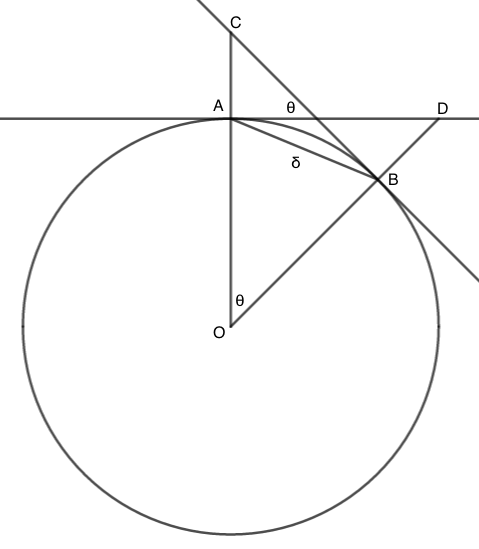
\includegraphics[width=\textwidth]{Circle-1.png}
    \caption{Drawing for Theorem 3.2.2}
  \end{subfigure}
  \begin{subfigure}[b]{0.32\textwidth}
    \centering
    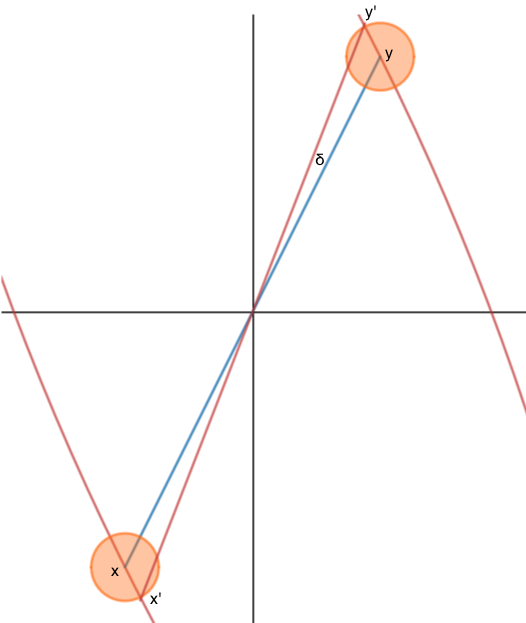
\includegraphics[width=\textwidth]{convex-1.png}
    \caption{Drawing for Theorem 3.2.3}
  \end{subfigure}
  \begin{subfigure}[b]{0.32\textwidth}
    \centering
    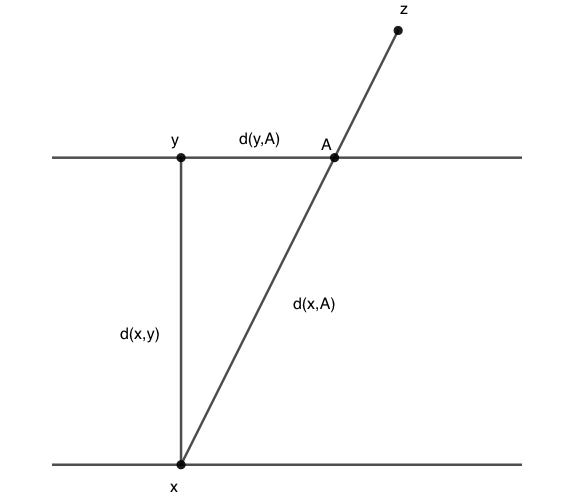
\includegraphics[width=\textwidth]{line-1.png}
    \caption{Drawing for Lemma 3.2.1}
  \end{subfigure}  
\end{figure}
\begin{theorem}
If $K\subset \mathbb{R}^2$ is compact and convex, then $R_K(\theta)$ is continuous.
\end{theorem}
\begin{proof}
For let $K$ be compact and convex, and without loss of generality suppose it contained within the unit disc and contains the origin. Let $\theta\in (0,2\pi)$ be given and let $\ell_{\theta}$ be a line through the origin making an angle $\theta$ with the horizontal. Let $x=(x_1,x_2),y=(y_1,y_2)\in K$ be such that $W_{\ell_{\theta}}(K) = d(x,y)$. Such points exist as $K$ is compact. Let $\varepsilon>0$ be given. About $x$, consider $B_{\frac{\varepsilon}{2}}(x)$, and similarly $B_{\frac{\varepsilon}{2}}(y)$. Neither of these are empty, as $K$ is convex. Let $x',y'\in K\cap(B_{\frac{\varepsilon}{2}}(x)\cup B_{\frac{\varepsilon}{2}}(y))$ be such that $d(x',y')$ is maximized. As this set is compact, such points exist. Let $\delta = \min\{|\theta-\frac{x_2'}{\sqrt{x_1'^2+x_2'^2}}|,|\theta-\frac{y_2'}{\sqrt{y_1'^2+y_2'^2}}|\}$. Then for $|\theta-\theta_0|<\delta$, $d(x,y)-\varepsilon \leq W_{\ell_{\theta_0}}(K)\leq d(x,y)+\varepsilon$, and thus $|W_{\ell_\theta}(K)-W_{\ell_{\theta_0}}(K)| < \varepsilon$.
\end{proof}
\begin{lemma}
If $K$ is a compact subset of $\mathbb{R}^2$ and $x,y\in K$ such that $d(x,y)=D(K)$, then the lines perpendicular to $\overline{xy}$ at $x$ and $y$ contain all of $K$ in between.
\end{lemma}
\begin{proof}
Suppose not. Let $\overline{X}$ be the line perpendicular to $\overline{xy}$ containing point $x$, and similarly define $\overline{Y}$. Suppose there is a point $z\in K$ that falls on the exterior of the region $\mathcal{U} = \{(x,y)\in \mathbb{R}^2: (x,y)\ \textrm{Lies Between } \overline{X}\ \textrm{and } \overline{Y}\}$. Note that $d(x,z)\ne d(y,z)$, as then $z$ would line between these two lines. Suppose $d(y,z)<d(x,z)$. Where the line $\overline{xz}$ cuts $\overline{Y}$ denote as $A$. But then $d(x,z) > d(x,A) = \sqrt{d(y,A)^2+d(x,y)^2}\geq d(x,y)$. A contradiction as $d(x,y) = D(K)$. Thus $z\in \mathcal{U}$.
\end{proof}
\begin{theorem}
If $K\subset \mathbb{R}^2$ is compact and convex, then there are points $x,y\in K$ such that $\check{W}(K)=d(x,y)$.
\end{theorem}
\begin{proof}
As $f_K(\theta)$ is continuous for convex compact set, and as it is continuous on a compact set $[0,2\pi]$, it attains its maximum. Let $\theta$ be such a maximum. Let $\ell_{\theta}$ be the line through the origin which makes an angle $\theta$ with the horizontal axis and consider set $K_{\ell_{\theta}}$. As $K$ is compact and $\ell_{\theta}$ is closed, $K_{\ell_{\theta}}$ is compact. Then $W=\{d(x,y):x,y\in K_{\ell_{\theta}}\}$ is bounded, has a least upper bound, and therefore there are points $x,y \in K$ such that $\check{W}(K)=d(x,y)$.
\end{proof}
\begin{theorem}
If $K$ is a compact convex set of $\mathbb{R}^2$, then $D(K) = \check{W}(K)$.
\end{theorem}
\begin{proof}
As $K$ is compact, $D(K)$ and $\check{W}(K)$ exists and there are points $x,y$ such that $d(x,y) = D(K)$ and points $x',y'$ such that $d(x',y') = \check{W}(K)$. Suppose $d(x',y')> d(x,y)$. A contradiction, as $d(x,y)$ is the diameter of $K$. So $d(x,y) \geq d(x',y')$. Now suppose $d(x,y)>d(x',y')$. But as $d(x',y')= \check{W}(K)$, $d(x',y')$ is the greatest length of any line segment that terminates in $K$ and such that perpendiculars at these terminating points contain all of $K$. But as $d(x,y)=D(K)$, the lines perpendicular to $\overline{xy}$ at $x$ and $y$ contain all of $K$, a contradiction. Thus $d(x',y') \geq d(x,y)$. But it was just showed that $d(x,y)\geq d(x',y')$. Thus, $d(x,y) = d(x',y')$. $D(K) = \check{W}(K)$.
\end{proof}
\begin{definition}
If $Q$ is a convex polygon with interior (That is, positive area) in $\mathbb{R}^2$, then the perimeter of $Q$ is the sum of the lengths of its edges. 
\end{definition}
\begin{definition}
The perimeter of a line segment $e$ is $P(e) = 2|e|$.
\end{definition}
\begin{remark}
This is for the sake of continuity. If we take a rectangle of length $|e|$ and width $\frac{1}{n}$, then the perimeter is $2|e|+\frac{2}{n} \rightarrow 2|e|$ as $n\rightarrow \infty$. Thus, for the puprose of continuity we define the perimeter of line segments to be twice their length.
\end{remark}
\begin{theorem}[Cauchy's Perimeter Theorem]
If $K$ is a compact convex subset of the plane, then $P(K) = \pi W(K)$.
\end{theorem}
\begin{proof}
Suppose that $Q$ is a convex polygon with edges $e_1,\hdots, e_n$. At each $e_i$, let $\theta_i$ be the angle made with $e_i$ and the horizontal axis of $\mathbb{R}^2$. The mean width is $W(Q) = \frac{1}{2\pi}\int_{0}^{2\pi} W_{\ell_\theta}(Q)d\theta = \frac{1}{2\pi} \int_{0}^{2\pi} \frac{1}{2} \sum_{i=1}^{n} |e_i||\cos(\theta-\theta_i)|d\theta = \frac{1}{4\pi}\sum_{i=1}^{n} |e_i|\int_{0}^{2\pi} |\cos(\theta-\theta_i)|d\theta = \frac{1}{\pi} \sum_{i=1}^{n} |e_i| = \frac{1}{\pi} P(Q)$. Thus, $P(Q) = \pi W(Q)$. For any convex compact subset $K\subset \mathbb{R}^2$, we may find a polygon $Q$ that approximates the boundary with a perimeter $P(Q)$ that is as close to $P(K)$ and a width $W(Q)$ as close to $W(K)$ as desired. That is, for all $n\in \mathbb{N}$, we can obtain a polynomial $Q_n$ such that $\max\{|W(Q_n)-W(K)|,|P(K)-P(Q_n)|\}< \frac{1}{n}$. Then $|P(K)-\pi W(K)| = |P(K) - P(Q_n)+P(Q_n)-\pi W(Q_n)+\pi W(Q_n)-\pi W(K)| \leq |P(K)-P(Q_n)|+|P(Q_n)-\pi W(Q_n)|+\pi|W(Q_n)-W(K)| < \frac{1}{n} + 0 + \frac{\pi}{n} = \frac{1+\pi}{n} \rightarrow 0$. Thus, $P(K) = \pi W(K)$ for arbitrary convex compact subsets of the plane.
\end{proof}
\begin{theorem}
There exist compact path-connected sets $K\subset \mathbb{R}^2$ such that $P(K) \ne \pi W(K)$.
\end{theorem}
\begin{proof}
Consider the set $K = \{(x,y) \in \mathbb{R}^2: x^2+y^2=1, y\geq 0\}$. Then $P(K) = 2\pi$, but \\ $W(K) = \pi(\pi+2)$. To see this, consider the set $\mathcal{K} = \{(x,y)\in \mathbb{R}^2: x^2 + y^2 \leq 1, y\geq 0\}$. This is convex and has perimeter $\pi+2$ and therefore $W(\mathcal{K}) = \pi(\pi+2)$. But, as the image shows, $W(K) = W(\mathcal{K})$. That is, $W_{\ell_{\theta}}(K)$ is the length of the line segment $\overline{AB}$, as is $W_{\ell_{\theta}}(\mathcal{K})$. Therefore the averages $W(K)$ and $W(\mathcal{K})$ are the same. Thus, $P(K) \ne \pi W(K)$.
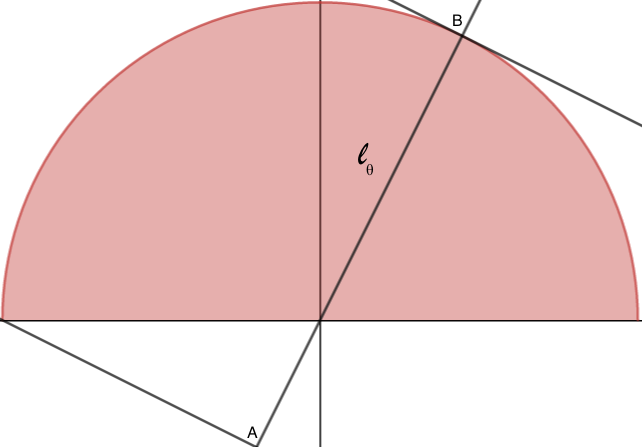
\includegraphics[scale=0.3]{semicircle-1.png}
\end{proof}
\begin{definition}
A functional $f$ with respect to subset inclusion is said to be monotonic on a family of sets $\mathscr{P}$ if and only if $f(K)\leq f(L)$ for all $K,L \in \mathscr{P}$ such that $K\subset L$.
\end{definition}
\begin{theorem}
If $K\subset L \in \mathscr{K}_2$, then $W_{\ell}(K) \leq W_{\ell}(L)$.
\end{theorem}
\begin{proof}
For let $\pi_{\ell}:\mathbb{R}^2 \rightarrow \ell$ be the orthogonal projection map of $\mathbb{R}^2$ to $\ell$. Then $\pi_{\ell}(K)\leq \pi_{\ell}(L)$ as $K\subset L$, and thus $W_{\ell}(K)\leq W_{\ell}(L)$.
\end{proof}
\begin{theorem}
If $K\subset L\in \mathscr{K}_2$, then $W(K)\leq W(L)$.
\end{theorem}
\begin{proof}
For $W_{\ell}(K)\leq W_{\ell}(L)$, and thus $W(K)=\frac{1}{2\pi}\int_{0}^{2\pi}W_{\ell_{\theta}}(K)d\theta \leq \frac{1}{2\pi}\int_{0}^{2\pi}W_{\ell_{\theta}}(L)d\theta=W(L)$.
\end{proof}
\begin{theorem}
If $K\subset L\in \mathscr{K}_2$, then $X_{\ell}(K)\leq X_{\ell}(L)$.
\end{theorem}
\begin{proof}
For if $x\in \ell\cap K$, then $x\in \ell\cap L$, and thus $X_{\ell}(K)=\mu(\ell\cap K) \leq \mu(\ell\cap L)=X_{\ell}(L)$.
\end{proof}
\begin{theorem}
If $K\subset L\subset \mathscr{K}_2$, then $D(K)\leq D(L)$.
\end{theorem}
\begin{proof}
For suppose not. Suppose $D(K)>D(L)$. Then, there are points $x,y\in K$ such that $d(x,y)> \sup\{d(x',y'):x',y'\in L\}$. But as $K\subset L$, $x,y\in L$ and thus $d(x,y) \not> \sup\{d(x',y'):x',y'\in L\}$. Thus, $D(K)\leq D(L)$.
\end{proof}
\begin{theorem}
If $K\subset L \subset \mathscr{K}_2$, then $R_K\leq R_L$.
\end{theorem}
\begin{proof}
For suppose not. Suppose $R_K>R_L$. But as $K\subset L$, either this circle contains all of $L$ as well or it doesn't. But then $R_L \not<R_K$. Thus, $R_L\geq R_K$.
\end{proof}
\begin{theorem}
If $K\subset L \in \mathscr{K}_2$, then $r_K \leq r_L$.
\end{theorem}
\begin{proof}
For suppose not. Suppose $r_K> r_L$. But as the inscribed circle of radius $r_K$ fits entirely in $K$, and $K\subset L$, then it fits inside of $L$. But then $r_K \not > r_L$. Thus, $r_L \geq r_K$.
\end{proof}
\begin{theorem}
If $K,L\in \mathscr{K}_2$ and $K\subset L$, then $P(K)\leq P(L)$.
\end{theorem}
\begin{proof}
As $K\subset L\in  \mathscr{K}_2$, $W(K)\leq W(L)$. As $K$ and $L$ are convex, $P(K)=\pi W(K)$ and $P(L)=\pi W(L)$. Thus, $P(K) \leq \pi W(L) = P(L)$. Therefore, $P(K)\leq P(L)$.
\end{proof}
\begin{theorem}
There exists sets $K,L\subset \mathbb{R}^2$ such that $L$ is convex, $K\subset L$, yet $P(K)>P(L)$.
\end{theorem}
\begin{proof}
For let $L = \{(x,y)\in \mathbb{R}^2: x^2 + y^2 \leq 1\}$. Then $P(L) = 2\pi$. Let $K = \{(x,y)\in \mathbb{R}^2: -\sqrt{2}x\leq y \leq \sqrt{2}x,\frac{-1}{\sqrt{3}} \leq x \leq \frac{1}{\sqrt{3}} \lor \sqrt{2}x\leq y \leq -\sqrt{2}x,\frac{-1}{\sqrt{3}} \leq x \leq \frac{1}{\sqrt{3}} \}$. $P(K) = 4(1+ \sqrt{\frac{2}{3}}) \approx 7.26>2\pi$.
\end{proof}
\begin{figure}[H]
  \begin{subfigure}[b]{0.49\textwidth}
     \centering
    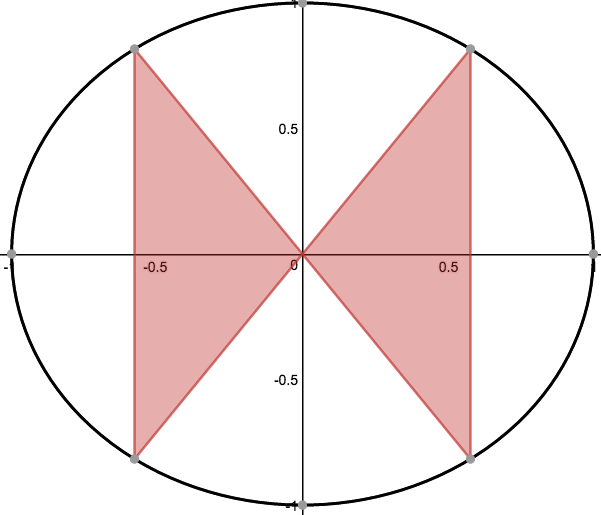
\includegraphics[width=\textwidth]{Circles-3.png}
    \caption{Drawing for Theorem 3.2.15}
  \end{subfigure}
  \begin{subfigure}[b]{0.49\textwidth}
    \centering
    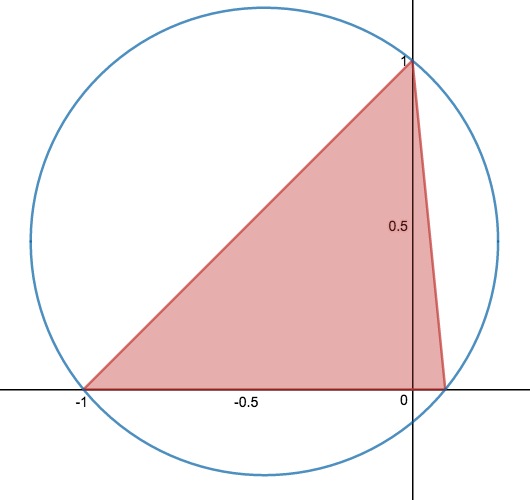
\includegraphics[width=\textwidth]{Circle-4.png}
    \caption{Drawing for Theorem 3.2.16}
  \end{subfigure}
\end{figure}
\begin{theorem}
There exist compact convex sets in $\mathbb{R}^2$ such that $D(K) < 2R_K$.
\end{theorem}
\begin{proof}
For consider the set $K=\{(x,y)\in \mathbb{R}^2: [0\leq y\leq x+1 \land x\geq 0]\lor [0\leq y\leq -10x+1\land x\geq 0]\}$. From Euclid, the smallest circle containing this triangle is the one defined by the three vertices (Three points define a triangle). This circle has the formula $(x+0.45)^2+(y-0.45)^2 = (0.45)^2 +(0.45+\frac{1}{10})^2$. Thus, $2R_K = \sqrt{0.45^2 +(0.45+\frac{1}{10})^2} > \sqrt{2} = D(K)$.
\end{proof}
\begin{theorem}
If $K$ is a compact convex set in $\mathbb{R}^2$, then $D(K) \leq 2R_K$.
\end{theorem}
\begin{proof}
For suppose not. Suppose $D(K) > 2R_K$. As $K$ is compact, there are points $x$ and $y$ in $K$ such that $d(x,y)=D(K)$. But then $d(x,y)>2R_K$, and thus at least one of $x$ or $y$ is not contained in the circle. A contradiction. Thus $D(K)\leq 2R_K$.
\end{proof}
\begin{theorem}
If $K$ is a compact convex set in $\mathbb{R}^2$, then $2\pi r_K \leq P(K)$.
\end{theorem}
\begin{proof}
From Calculus of Variations we know that the circle maximizes the area contained with a set of perimeter $p$. As the inscribed circle has perimeter $2\pi r_K$ and as the circle is a subset of $K$, it is true that $A(K)$ is greater than or equal the area of the circle. Thus, $P(K)\geq 2\pi r_K$.
\end{proof}
\begin{theorem}
For a compact convex set of $\mathbb{R}^2$, $P(K) \leq 2\pi R_K$.
\end{theorem}
\begin{proof}
As $K$ is convex, $P(K) = \pi W(K) \leq \pi \check{W}(K) = \pi D(K) \leq 2\pi R_K$.
\end{proof}
\begin{theorem}
If $K$ is a compact and convex subset of $\mathbb{R}^2$, then $2D(K)\leq P(K)$.
\end{theorem}
\begin{proof}
Suppose not. Suppose $2D(K) >P(K)$. As $K$ is compact and convex, there exist points $x,y\in K$ such that $d(x,y) = D(K)$. But as $K$ is convex, the line contained between $x,y$ in contained in $K$. Thus, $P(\overline{xy}) = 2D(K)$. But as $\overline{xy}\subset K$, $P(K)>P(\overline{xy})$, a contradiction. Thus, $2D(K) \leq P(K)$.
\end{proof}
\begin{theorem}
There exist compact convex subsets of $\mathbb{R}^2$ such that $2D(K) = P(K)$.
\end{theorem}
\begin{proof}
For take a straight line segment of length $\ell$. Then $D(K) = \ell$, $P(K) = 2\ell$, and thus $2D(K) = P(K)$.
\end{proof}
\begin{theorem}
If $K$ is a compact convex subset of $\mathbb{R}^2$, then $P(K) \leq \pi D(K)$.
\end{theorem}
\begin{proof}
From Cauchy's Perimeter theorem, $P(K) = \pi W(K) \leq \pi \check{W}(K) = \pi D(K)$.
\end{proof}
\begin{theorem}
For a compact convex subset $K$ of $\mathbb{R}^2$, $P(K) = \pi D(K)$ if and only if $W_{\ell}(K)$ is a constant.
\end{theorem}
\begin{proof}
For then $\frac{1}{2\pi} \int_{0}^{2\pi} W_{\ell_{\theta}}(K) d\theta = \check{W}(K)$. But as $W_{\ell_{\theta}}(K)$ is continuous for compact convex bodies, it must be true that $W_{\ell_{\theta}}(K) = \check{W}(K)$ for all $\ell_{\theta}$. Thus, $K$ is of constant width.
\end{proof}
\begin{remark}
There are many types of shapes that have constant width besides discs. The Reuleaux Triangle is such an example.
\end{remark}
Triangles are the simplest convex bodies in the plane other than points and lines. Any convex polygon can be written as the union of triangles with disjoint interiors. 
\begin{theorem}
If $\Delta_s$ is an equilateral triangle with edge length $s$, then $\Delta_s$ has the following properties:
\begin{enumerate}
\begin{multicols}{5}
\item $A(\Delta_s) = \frac{\sqrt{3}}{4}s^2$
\item $P(\Delta_s) = 3s$
\item $W(\Delta_s) = \frac{3s}{\pi}$
\item $R_{\Delta_s} = \frac{1}{\sqrt{3}}s$
\item $r_{\Delta_s} = \frac{1}{2\sqrt{3}}s$
\end{multicols}
\end{enumerate}
\end{theorem}
\begin{proof}
In order:
\begin{enumerate}
    \item From Pythagoras, $A(\Delta_s) =2\times\big[\frac{1}{2}(\frac{1}{2}s)(\frac{\sqrt{3}}{2}s)\big] = \frac{\sqrt{3}}{4}s^2$
    \item There are three edges, each of length $s$, and thus $P(\Delta_s) = 3s$.
    \item $W(\Delta_s) = \frac{1}{\pi}P(\Delta_s) = \frac{3s}{\pi}$
    \item The circumcircle gives the following equations:
    \begin{enumerate}
        \item $R_{\Delta_s}^2=\frac{s^2}{4}+h^2$
        \item $h+R_{\Delta_s} = \frac{\sqrt{3}}{2}s$
    \end{enumerate}
    This has solution $R_{\Delta_s}=\frac{1}{\sqrt{3}}s$
    \item $r_{\Delta_s} = \frac{R_{\Delta_s}}{2}= \frac{1}{2\sqrt{3}}s$
\end{enumerate}
\end{proof}
\begin{theorem}
If $T$ is a triangle in the plane, then there is a linear transformation $\psi$ such that $\psi T$ is equilateral.
\end{theorem}
\begin{proof}
For let $T$ be a triangle with vertices $a=(x_1,y_1)$, $b=(x_2,y_2)$, $c=(x_3,y_3)$. Let $A = d(b,c)$, $B=d(a,c)$, and $C=d(a,b)$. Suppose If $A=B=C$, we are done. Thus, suppose $C\geq B >A$. At point $a$ and with radius $C$, construct the circle $b,c',d$, and point $b$ and with radius $C$, construct the circle $a,c',e$. If we can shift $c$ to $c'$ in a linear fashion, we are done. Let $\psi =$
\end{proof}
\begin{theorem}
If $T$ is a triangle with edges $a,b,c$ and opposite angles $\alpha,\beta,\gamma$, respectively, then $A(T) = \frac{\sin(\alpha)}{2}bc = \frac{\sin(\beta)}{2}ac = \frac{\sin(\gamma)}{2}ab$
\end{theorem}
\begin{proof}
Suppose the triangle is acute. The proof is symmetric for all sides, so we prove it for just $\alpha$. Note that the perpendicular $h$ dropped from the vertex of $a$ onto $b$ satisfies $h^2+\ell_1^2 = c^2$ and $h^2+\ell_2^2 = a^2$, where $\ell_1+\ell_2 = b$. Then $\sin(\alpha) = \frac{h}{c}$ and $A(T) = \frac{1}{2}h\ell_1 + \frac{h}{2}h\ell_2 = \frac{h}{2}(\ell_1+\ell_2)h = \frac{1}{2}bh = \frac{1}{2}bc\sin(\alpha)$. An identical argument works for obtuse triangles.
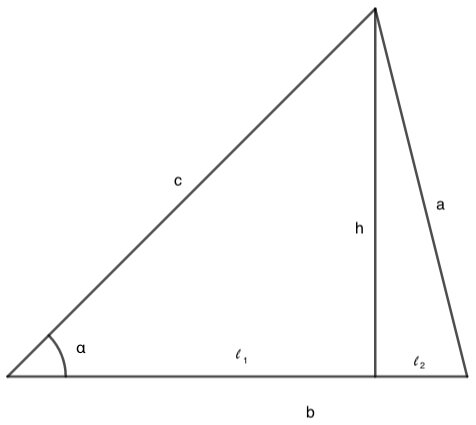
\includegraphics[scale=0.3]{triangle-1.png}
\end{proof}
\begin{corollary}[The Law of Sines]
For a triangle with edges $a,b,c$ and opposite angles $\alpha,\beta,\gamma$, $\frac{\sin(\alpha)}{a} = \frac{\sin(\beta)}{b} = \frac{\sin(\gamma)}{c}$
\end{corollary}
\begin{proof}
From the previous theorem, divide by $\frac{abc}{2}$ to obtain the result.
\end{proof}
\begin{theorem}[The Law of Cosines]
Given a triangle with lengths $a,b,c$ and opposite edges $\alpha,\beta,\gamma$, $c^2=a^2+b^2-2ab\cos(\gamma)$.
\end{theorem}
\begin{proof}
If $\gamma=\frac{\pi}{2}$, this is Pythagoras' Theorem. Thus, suppose $0<\gamma < \frac{\pi}{2}$. Where $c$ and $a$ meet, drop a perpendicular onto $c$ and call this $h$. $h$ satisfies $h^2+\ell_1^2 = c^2$ and $h^2+\ell_2^2=a^2$ from Pythagoras' Theorem, where $\ell_1+\ell_2 = b$. But $\ell_2 = a\cos(\gamma)$, so $\ell_1 = b-a\cos(\gamma)$. Thus $c^2 = h^2 + b^2 +a^2\cos^2(\gamma)-2ab\cos(\gamma)$. But $h = a\sin(\gamma)$. Thus, $c^2 = b^2 + a^2 \cos^2(\gamma)+\sin^2(\gamma)-2ab\cos(\gamma) = b^2 + a^2(\sin^2(\gamma)+\cos^2(\gamma))-2ab\cos(\gamma) = a^2 + b^2 -2ab\cos(\gamma)$. A similar construction is done if $\frac{\pi}{2}<\gamma < \pi$.
\end{proof}
\begin{theorem}
Given a triangle $\Delta$ with lengths $a\leq b\leq c$, $D(\Delta)=c$.
\end{theorem}
\begin{proof}
At the midpoint of $c$, and with radius $c$, construct a circle. This circle contains the entirety of $\Delta$, and thus for all points $x,y\in \Delta$, $d(x,y)\leq c$. Thus, $c=D(\Delta)$.
\end{proof}
\begin{theorem}[Heron's Formula]
For a triangle with lengths $a,b,c>0$, $A(T)^2 = \frac{1}{16}(a+b+c)(-a+b+c)(a-b+c)(a+b-c)$.
\end{theorem}
\begin{proof}
For $A(T) = \frac{1}{2}ab \sin(\gamma) = \frac{1}{2}ab\sqrt{1-\cos^2(\gamma)} = \frac{1}{4}\sqrt{4a^2 b^2 - (a+b-c)^2}=\\ \frac{1}{4}\sqrt{(2ab-(a^2+b^2-c^2))(2ab+(a^2+b^2+c^2))} = \frac{1}{4}\sqrt{(c^2-(a-b)^2)((a+b)^2-c^2)} = \\ \frac{1}{4}\sqrt{(a+b+c)(-a+b+c)(a-b+c)(a+b-c)}$. Squaring this gives the result.
\end{proof}
\begin{theorem}
For any triangle $\Delta$, $r_{\Delta}P(\Delta) = 2A(\Delta)$.
\end{theorem}
\begin{proof}
For let $\Delta$ has sides $a,b,c$, with opposite angles $\alpha, \beta, \gamma$, respectively. Then $A(\Delta) = \frac{ab}{2}\sin(\gamma)$ and $P(\Delta)=a+b+c$. Thus, $\frac{2A(\Delta)}{P(\Delta)} = \frac{ab\sin(\gamma)}{a+b+c}$. But this is the radius of the incircle of $\Delta$. Therefore, etc.
\end{proof}
\begin{theorem}[Viviani's Theorem: Page 17]
\end{theorem}
\begin{theorem}
There exist convex polygon's such that the inradius is not unique.
\end{theorem}
\begin{proof}
For consider the rectangle $[0,2]\times [0,1]$. The diameter of any circle that sits inside this body must be at most $1$, and thus the radius is at most $\frac{1}{2}$. However, there are multiple circles that achieve this. For example $(x-\frac{1}{2})^2+(y-\frac{1}{2})^2=\frac{1}{2}$ and $(x-\frac{3}{2})^2+(y-\frac{3}{2})^2=\frac{1}{2}$.
\end{proof}
\begin{theorem}
For an acute triangle, $\frac{2(A)}{abc} = \frac{1}{R_T}$.
\end{theorem}
\begin{theorem}
If $\Delta$ is a triangle with vertices $A,B,C$ and sides $a,b,c$, then given a circle that contains $A,B,C$, the radius of this circle $R$ satisfies $\frac{1}{R} =\frac{2A(\Delta)}{abc}$
\end{theorem}
\begin{definition}
If $K\in \mathscr{K}_2$, then $-K = \{-x:x\in K\}$.
\end{definition}
\begin{theorem}
If $K\in \mathscr{K}_2$, then $W_{\ell}(K) = W_{\ell}(-K)$.
\end{theorem}
\begin{proof}
For let $x,y\in K$ be such that $d(x,y) = W_{\ell}(K)$. Then $d(-x,-y) = W_{\ell}(-K) = d(x,y)$. Therefore, etc.
\end{proof}
\begin{theorem}
There exist sets $K$ and $L$ such that $W_{\ell}(K)<W_{\ell}(L)$ for all $\ell$ yet $K\not\subset L$ for any translation or rotation of $K$.
\end{theorem}
\begin{definition}
For $K\in \mathscr{K}$ and unit vector $u$, $\bar{X}_{u}(K)$ is the mean value of $X_{\ell}(K)$ over all lines $\ell$ parallel to $u$ such that $X_{\ell}(K)>0$.
\end{definition}
\begin{theorem}
For $K\in \mathscr{K}_2$, $\bar{X}_{u}(K) = W_{\ell}(K)=A(K)$.
\end{theorem}
\end{document}